
\chapter{Evaluierung von Net2Net}\label{sec:net2netexperimente}
Die Operatoren zur Beschleunigung des Lernens durch Wissenstransfer werden in diesem Kapitel evaluiert. Diese Evaluierung arbeitet mit einer selbst erstellten Implementierung auf Grundlage der Veröffentlichung zum Thema Net2Net \cite{net2net}.

Die Evaluierung umfasst drei unterschiedliche Situationen, diese Situation sind ähnlich, wie in der dazugehörigen Quelle \cite{net2net}. Die Evaluierung arbeitet mit einem ResNet, wie in Kapitel \ref{sec:baseline}. In der Veröffentlichung wird mit einem Inception Net gearbeitet. Das Inception Netz wird in Kapitel \ref{sec:inception} vorgestellt.

In der ersten Situation wird der Operator für ein breiteres Netz evaluiert, in dem das Netz breiter gemacht wird. 
In der zweiten Situation wird der Operator für ein tieferes Netz benutzt um zusätzliche Blöcke hinzuzufügen oder bestehenden Blöcken Schichten hinzuzufügen. In der dritten Situation werden beide Operatoren kombiniert. Mit der Kombination wird der Raum der möglichen Operatoranwendungen erkundet, ausgehend von einem Modell.
Die drei Situationen werden in den drei folgenden Unterkapiteln näher beschrieben. Anpassungen der Lernrate werden hier nicht vorgenommen.

\section{Evaluierung des Operators für ein breiteres Netz}
Der Operator für ein breiteres Netz wird evaluiert, in dem ein schmalles Baseline-Netz für 90 Epochen trainiert wird. Dann wird der Operator angewendet. Nach der Anwendung wird für weitere 90 Epochen trainiert. Der Operator für ein breiteres Netz macht das Netz für diese Evaluierung doppelt so breit.


Wie in Kapitel \ref{sec:net2net} beschrieben werden beim Operator für ein breiteres Netz die Gewichte für die neu hinzugefügten Gewichte aus den ursprünglichen Gewichten ausgewählt und so normalisiert, dass die approximierte Funktion nach Anwendung des Operators nicht signifikant von der approximierten Funktion mit den neuen Gewichten abweicht. Um zu evaluieren wie gut diese Methode funktioniert wird sie auf das schmalle Baseline Netz angewendet und verglichen mit dem schmallen und breiten Baseline-Netz. Um die Methode der Initialisierung der zusätzlichen Kanäle zu evaluieren wird als Vergleich ein Netz trainiert, bei welchem die zusätzlichen Gewichte zufällig initialisiert werden.
\begin{figure}
     \centering
     \subfloat[][]{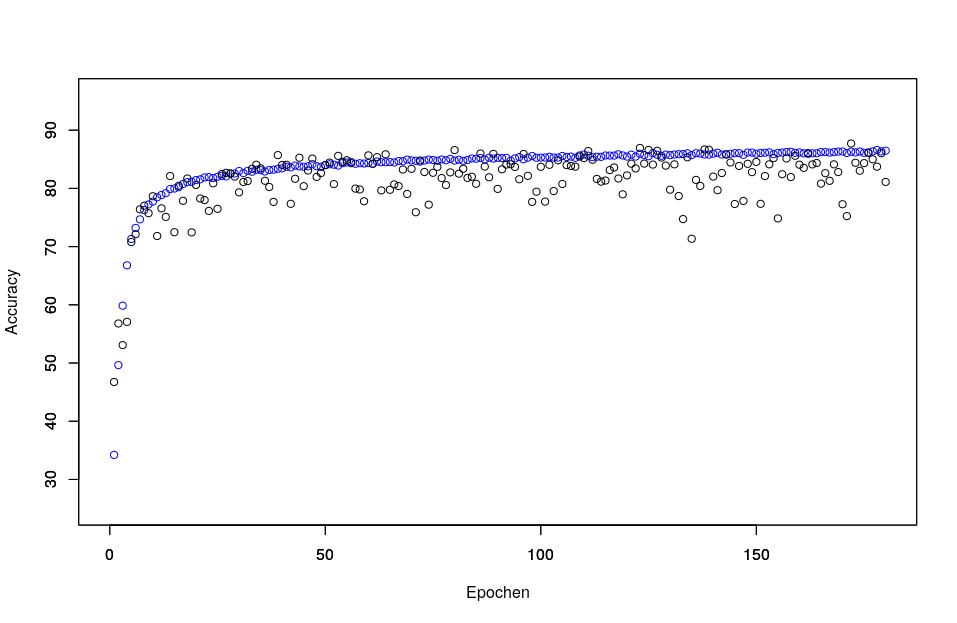
\includegraphics[width= .47\textwidth]{KapitelPartB/Images/wider1.png}\label{abb:wider1}}     
     \subfloat[][]{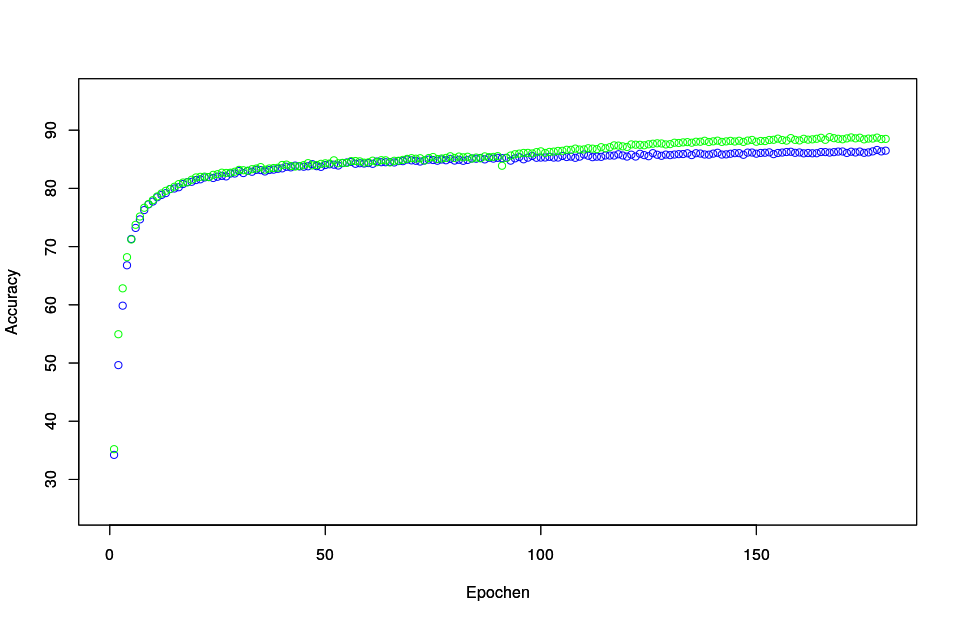
\includegraphics[width= .47\textwidth]{KapitelPartB/Images/wider2.png}\label{abb:wider2}}
     \hfill
     \subfloat[][]{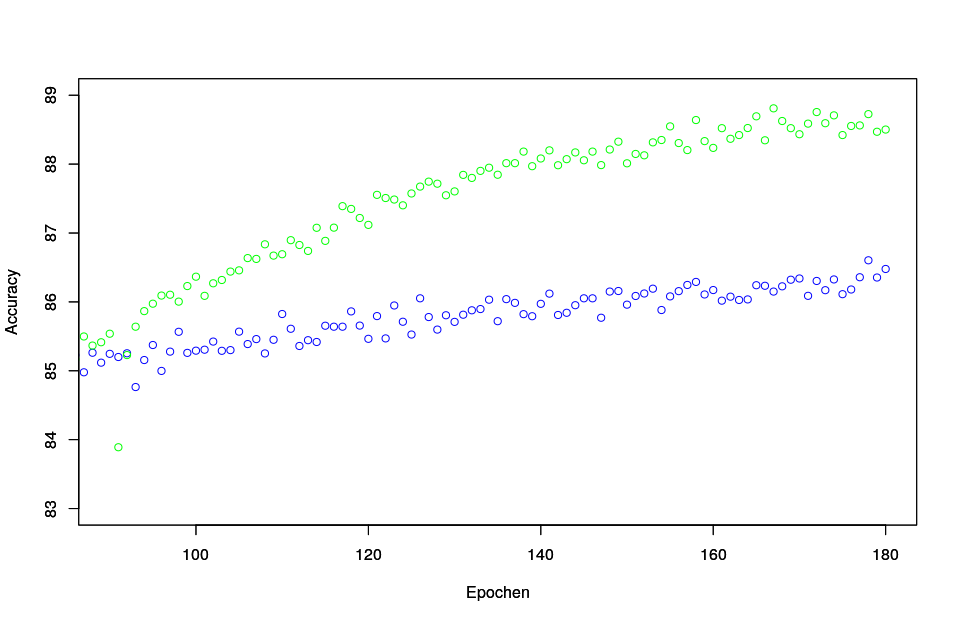
\includegraphics[width= .47\textwidth]{KapitelPartB/Images/wider3.png}\label{abb:wider3}}
     \subfloat[][]{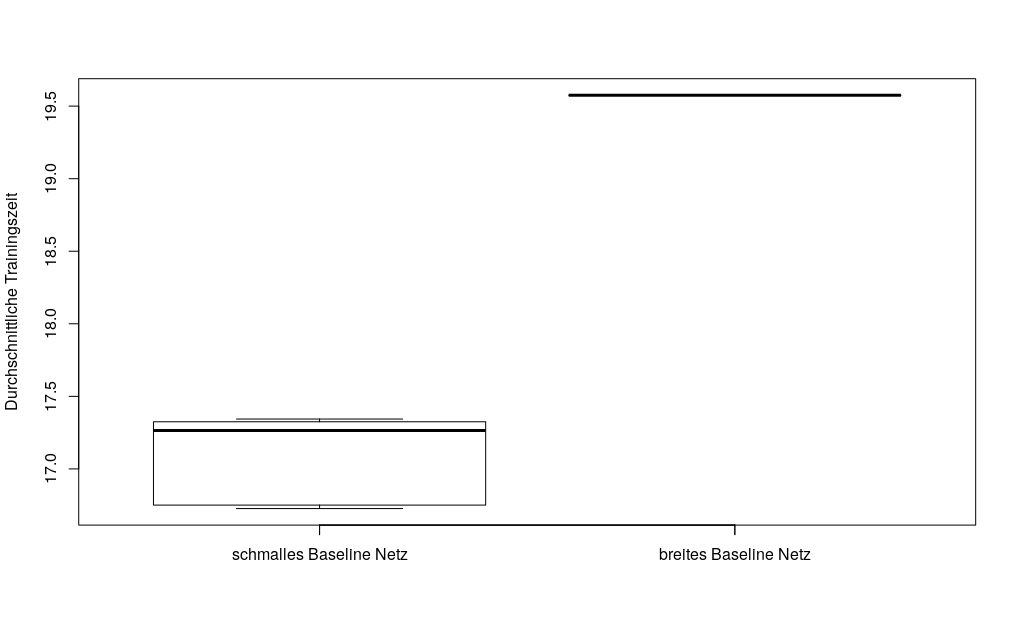
\includegraphics[width= .47\textwidth]{KapitelPartB/Images/baselineS.png}\label{abb:wider4}}
     
     \caption{}
     \label{abb:wider}
\end{figure}

In Abbildung \ref{abb:wider1} ist der Verlauf der Accuracy des schmallen Baseline Netzes in blau und des breiten Baseline Netzes in schwarz über 180 Epochen ohne Anpassung der Lernrate zu sehen. Es fällt auf, dass das schmalle Baseline Netz währenddem Training wesentlich stabiler trainiert als das breite. Allerdings ist das schmalle Baseline-Netz nach wenigen Epochen bereits so weit, dass es kaum Verbesserungen gibt. Auf das schmalle Baseline Netz wird im nächsten Schritt der Operator für ein breiteres Netz angewendet. In Abbildung \ref{abb:wider2} ist der Verlauf der Accuracy des schmallen Baseline Netzes in blau im Vergleich zum schmallen Baseline Netz mit Anwendung des Operators in grün zu sehen. In Abbildung \ref{abb:wider3} ist ein Ausschnitt von Abbildung \ref{abb:wider2} für die Epochen 90 -180 zu sehen. An den beiden Grafiken ist eindeutig abzulesen, dass der Operator für ein breiteres Netz auf dem Baseline Netz die Accuracy verbessert. Die Verbesserung liegt bei den verglichenen Durchläufen bei 2 \%. 

Gegenüber dem breiten Baseline Netz spart dieses Training mit dem Operator dadurch Zeit, dass in den ersten 90 Epochen weniger Trainingszeit verbraucht wird. In Abbildung \ref{abb:wider4} ist die durchschnittliche Trainingszeit des schmallen Baseline Netz verglichen mit dem breiten in einem Boxplot zu sehen. Bei der hier verwendeten Größe des Netzes dauert die Anwendung des Operators für ein breiteres Netz etwa 0,3 Sekunden. Damit liegt die Trainingszeit des Netzes mit Anwendung des Operators zwischen schmallen und breiten Baseline-Netz.


Bei dem hier verwendeten Netz und Datensatz macht die Anwendung des Operators Sinn, dass sie das Training stabiler, schneller und besser macht.





\section{Evaluierung des Operators für ein tieferes Netz}
Zur Evaluierung des Operators für ein tieferes Netz wird zunächst wie in der Veröffentlichung jeder Block um eine Schicht erweitert. Dafür wird mit einem Netz gestartet, welches jeweils nur eine Convolution und Batchnormalisation Schicht pro Block hat $ (l=1)$. 

Dabei werden die zusätzlichen Schichten wie in Kapitel \ref{sec:net2net} beschrieben initialisiert. Als Vergleich dient das Baseline-Netz aus Kapitel \ref{sec:baseline}. Ein weiterer Vergleichspunkt ist das Netz, mit welchem trainiert wird beovr der Operator abgewendet wird. Dieses Netz wird zusätzlich über 180 Epochen trainiert, um die Auswirkungen des Operators zu sehen. Die Accuracy des Ausgangsnetzes ist in Abbildung \ref{abb:deeper11} zu sehen. Zu beobachten ist, dass das Augangsnetz auch unstabil trainiert. 

\begin{figure}
     \centering
     \subfloat[][]{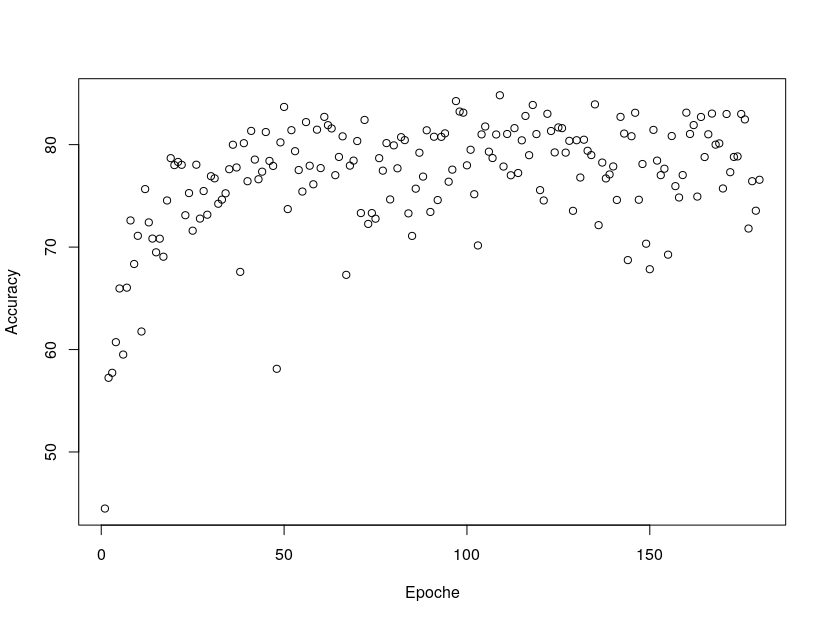
\includegraphics[width= .47\textwidth]{KapitelPartB/Images/baselinel1.png}\label{abb:deeper11}}     
     \subfloat[][]{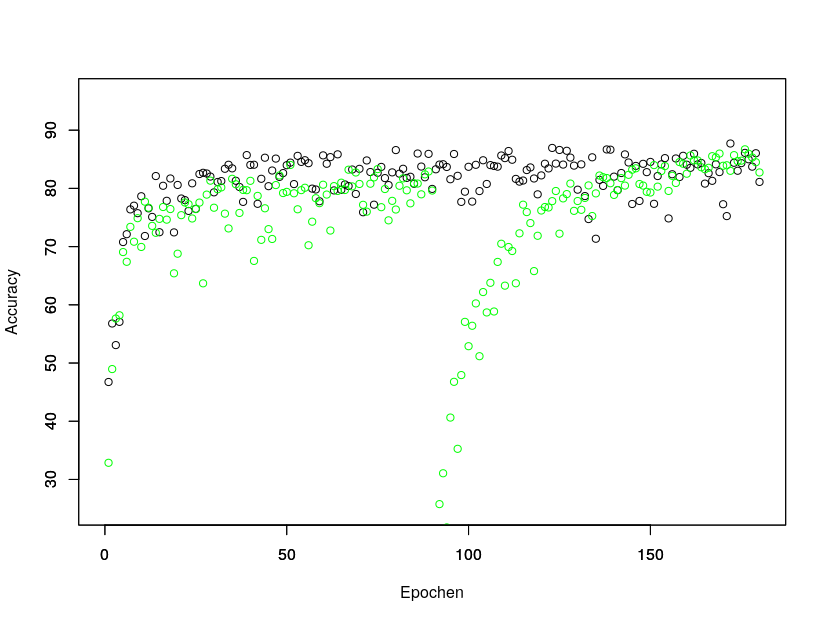
\includegraphics[width= .47\textwidth]{KapitelPartB/Images/deeper12.png}\label{abb:deeper12}}
     \hfill
     \subfloat[][]{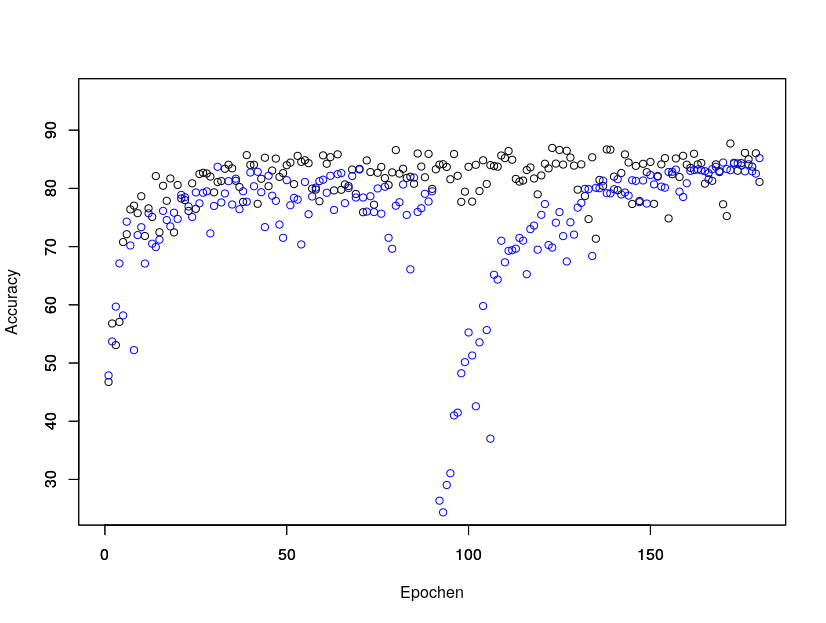
\includegraphics[width= .47\textwidth]{KapitelPartB/Images/deeper13.png}\label{abb:deeper13}}
     \subfloat[][]{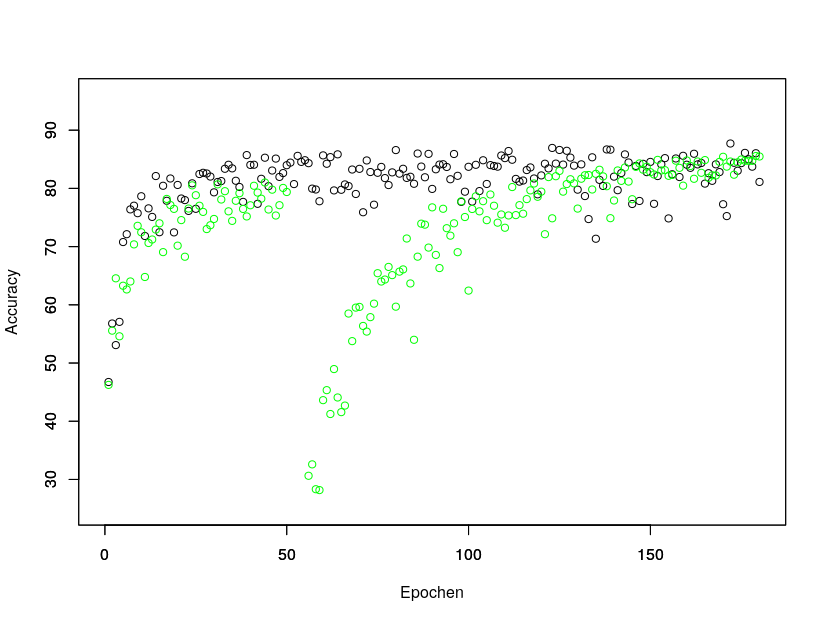
\includegraphics[width= .47\textwidth]{KapitelPartB/Images/deeper14.png}\label{abb:deeper14}}\\
     \subfloat[][]{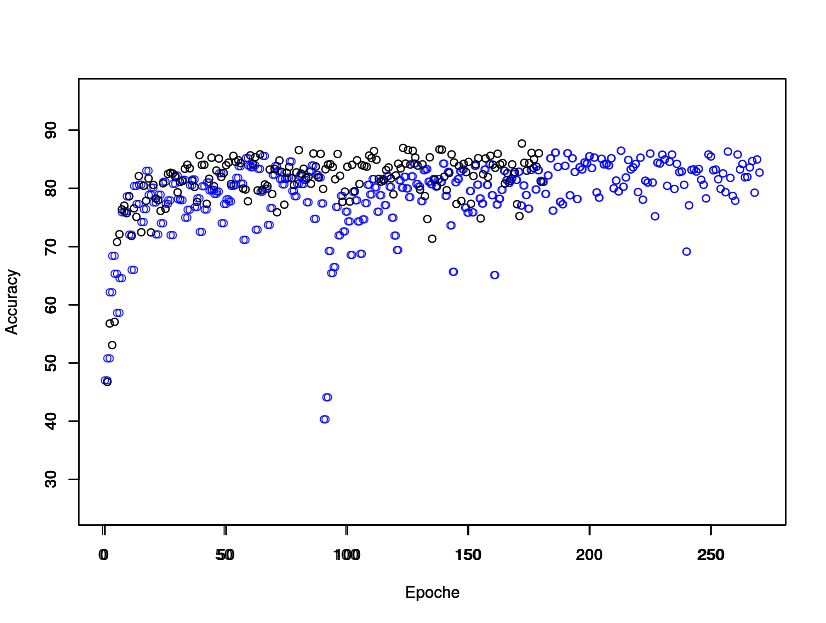
\includegraphics[width= .47\textwidth]{KapitelPartB/Images/deeper21.png}\label{abb:deeper21}}

     \caption{}
     \label{abb:deeper}
\end{figure}


Wird in Epoche 90 der Operator für ein tieferes Netz angewendet, so wird im Gegensatz zum Operator für ein breiteres Netz danach ein deutliches Abfallen der Accuracy auf unter 30 \% beobachtet. Allerdings lässt sich hier auch eine leicht erhöhte Stabilität des Trainings beobachten. In schwarz ist jeweils das Training des breiten Baseline Netzes zu sehen.  Dies ist Abbildung \ref{abb:deeper12} in grün abgebildet. Die blaue Kurve in Abbildung \ref{abb:deeper13} zeigt eine andere Initialisierungsmethode. Diese fügt zusätzlich noch eine normalverteilte Störung mit $\mu = 0, \sigma^2 = 0.1$ ,den Gewichten die gleich Null sind nach der Initialisierung, hinzu. 

Zu beobachten ist, dass das Netz von vorne anfängt zu trainieren. Trotz dieses Problem wird Zeit gespart, durch die schnellere Trainingszeit bis zum Anwenden des Operators. Da beim Ausgangsnetz bereits recht schnell keine Verbesserung auftritt zeigt Abbildung \ref{abb:deeper14} das Ergebnis bei Anwendung des Operators in Epoche 50 in Grün. 
Es zeigt sich, dass bei der Verwendung dieser Netzstruktur auf dem Datensatz Cifar10 keine wesentliche Verbesserung gegenüber der Netzstruktur nachdem Anwenden des Operators ergibt. Es ergibt sich jedoch eine Verbesserung gegenüber dem Ausgangsnetz und die Stabilität des Trainings steigt.



Eine weitere Verwendung des Operators für ein tieferes Netz ist die Möglichkeit einen neuen Block hinzuzufügen. Nur ein einfaches Hinzufügen würde hier zu Problemen führen, da durch das Hinzufügen eines Blockes die vom Netz berechnete Funktion von der vorher berechneten Funktion abweicht. Gelöst wird dies, in dem alle Blöcke vor der Addition mittels eines muliplikativen Faktors skaliert werden. Wie in Abbildung \ref{abb:diagramm} abgebildet ist, werden alle muliplikativen Faktoren des Ausgangsnetzes auf 1 gesetzt, sodass hier kein Effekt auf die berechnende Funktion entsteht. Beim neu hinzuzufügenden Block werden die beiden multiplikativen Faktoren auf 0,5 gesetzt. Die multiplikativen Faktoren sind trainierbar.

Da der neu hinzuzufügende Block ein Identitätsblock ist wird das Ergebnis des Identitätsblockes und der Kurzschlussverbindung zusammen keinen Effekt auf die vom Netz berechnete Funktion haben. In Abbildung \ref{abb:diagramm} ist zu sehen, wie der neue Block in das Gefüge der anderen Blocks passt.


In Abbildung \ref{abb:deeper21} ist abgebildet, wie sich die Accuracy eines Netzes mit den multiplikativen Faktoren über 180 Epochen verhält. Auch hier ergibt sich zwar eine Steigerung gegenüber dem Ausgangsnetz. Die Accuracy des Ausgangsnetzes ist in Abbilsung \ref{abb:BaselineMul} zu sehen.

Eine Verbesserung gegenüber dem Baseline Netz ergibt sich allerdings nicht. Wie auch schon beim 1. Operator für ein tieferes Netz ergibt sich eine Einsparung in der Trainingszeit.


\begin{figure}
     \centering
     \subfloat[][]{% Graphic for TeX using PGF
% Title: /home/j3ssi/Diagramm2.dia
% Creator: Dia v0.97+git
% CreationDate: Mon Dec 21 02:52:59 2020
% For: j3ssi
% \usepackage{tikz}
% The following commands are not supported in PSTricks at present
% We define them conditionally, so when they are implemented,
% this pgf file will use them.
\ifx\du\undefined
  \newlength{\du}
\fi
\setlength{\du}{15\unitlength}
\begin{tikzpicture}[even odd rule, scale=0.6]
\pgftransformxscale{1.000000}
\pgftransformyscale{-1.000000}
\definecolor{dialinecolor}{rgb}{0.000000, 0.000000, 0.000000}
\pgfsetstrokecolor{dialinecolor}
\pgfsetstrokeopacity{1.000000}
\definecolor{diafillcolor}{rgb}{1.000000, 1.000000, 1.000000}
\pgfsetfillcolor{diafillcolor}
\pgfsetfillopacity{1.000000}
\pgfsetlinewidth{0.100000\du}
\pgfsetdash{}{0pt}
\pgfsetmiterjoin
\pgfsetbuttcap
{\pgfsetcornersarced{\pgfpoint{0.000000\du}{0.000000\du}}\definecolor{diafillcolor}{rgb}{1.000000, 1.000000, 1.000000}
\pgfsetfillcolor{diafillcolor}
\pgfsetfillopacity{1.000000}
\fill (7.055000\du,8.390395\du)--(7.055000\du,11.190395\du)--(13.255000\du,11.190395\du)--(13.255000\du,8.390395\du)--cycle;
}{\pgfsetcornersarced{\pgfpoint{0.000000\du}{0.000000\du}}\definecolor{dialinecolor}{rgb}{0.000000, 0.000000, 0.000000}
\pgfsetstrokecolor{dialinecolor}
\pgfsetstrokeopacity{1.000000}
\draw (7.055000\du,8.390395\du)--(7.055000\du,11.190395\du)--(13.255000\du,11.190395\du)--(13.255000\du,8.390395\du)--cycle;
}\pgfsetlinewidth{0.100000\du}
\pgfsetdash{}{0pt}
\pgfsetbuttcap
{
\definecolor{diafillcolor}{rgb}{0.000000, 0.000000, 0.000000}
\pgfsetfillcolor{diafillcolor}
\pgfsetfillopacity{1.000000}
% was here!!!
\pgfsetarrowsend{stealth}
\definecolor{dialinecolor}{rgb}{0.000000, 0.000000, 0.000000}
\pgfsetstrokecolor{dialinecolor}
\pgfsetstrokeopacity{1.000000}
\draw (10.305000\du,3.490395\du)--(10.343500\du,8.340745\du);
}
\pgfsetlinewidth{0.100000\du}
\pgfsetdash{}{0pt}
\definecolor{diafillcolor}{rgb}{1.000000, 1.000000, 1.000000}
\pgfsetfillcolor{diafillcolor}
\pgfsetfillopacity{1.000000}
\pgfpathellipse{\pgfpoint{10.205000\du}{15.940392\du}}{\pgfpoint{1.325000\du}{0\du}}{\pgfpoint{0\du}{1.625000\du}}
\pgfusepath{fill}
\definecolor{dialinecolor}{rgb}{0.000000, 0.000000, 0.000000}
\pgfsetstrokecolor{dialinecolor}
\pgfsetstrokeopacity{1.000000}
\pgfpathellipse{\pgfpoint{10.205000\du}{15.940392\du}}{\pgfpoint{1.325000\du}{0\du}}{\pgfpoint{0\du}{1.625000\du}}
\pgfusepath{stroke}
\pgfsetlinewidth{0.100000\du}
\pgfsetdash{}{0pt}
\pgfsetbuttcap
{
\definecolor{diafillcolor}{rgb}{0.000000, 0.000000, 0.000000}
\pgfsetfillcolor{diafillcolor}
\pgfsetfillopacity{1.000000}
% was here!!!
\pgfsetarrowsend{stealth}
\definecolor{dialinecolor}{rgb}{0.000000, 0.000000, 0.000000}
\pgfsetstrokecolor{dialinecolor}
\pgfsetstrokeopacity{1.000000}
\draw (10.155000\du,11.190395\du)--(10.187367\du,14.265253\du);
}
\pgfsetlinewidth{0.100000\du}
\pgfsetdash{}{0pt}
\pgfsetbuttcap
{
\definecolor{diafillcolor}{rgb}{0.000000, 0.000000, 0.000000}
\pgfsetfillcolor{diafillcolor}
\pgfsetfillopacity{1.000000}
% was here!!!
\pgfsetarrowsend{stealth}
\definecolor{dialinecolor}{rgb}{0.000000, 0.000000, 0.000000}
\pgfsetstrokecolor{dialinecolor}
\pgfsetstrokeopacity{1.000000}
\draw (10.205000\du,17.565395\du)--(10.285000\du,21.597895\du);
}
\pgfsetlinewidth{0.100000\du}
\pgfsetdash{}{0pt}
\definecolor{diafillcolor}{rgb}{1.000000, 1.000000, 1.000000}
\pgfsetfillcolor{diafillcolor}
\pgfsetfillopacity{1.000000}
\pgfpathellipse{\pgfpoint{10.285000\du}{23.222895\du}}{\pgfpoint{1.325000\du}{0\du}}{\pgfpoint{0\du}{1.625000\du}}
\pgfusepath{fill}
\definecolor{dialinecolor}{rgb}{0.000000, 0.000000, 0.000000}
\pgfsetstrokecolor{dialinecolor}
\pgfsetstrokeopacity{1.000000}
\pgfpathellipse{\pgfpoint{10.285000\du}{23.222895\du}}{\pgfpoint{1.325000\du}{0\du}}{\pgfpoint{0\du}{1.625000\du}}
\pgfusepath{stroke}
\pgfsetlinewidth{0.100000\du}
\pgfsetdash{}{0pt}
\definecolor{diafillcolor}{rgb}{1.000000, 1.000000, 1.000000}
\pgfsetfillcolor{diafillcolor}
\pgfsetfillopacity{1.000000}
\pgfpathellipse{\pgfpoint{18.305000\du}{15.990392\du}}{\pgfpoint{1.325000\du}{0\du}}{\pgfpoint{0\du}{1.625000\du}}
\pgfusepath{fill}
\definecolor{dialinecolor}{rgb}{0.000000, 0.000000, 0.000000}
\pgfsetstrokecolor{dialinecolor}
\pgfsetstrokeopacity{1.000000}
\pgfpathellipse{\pgfpoint{18.305000\du}{15.990392\du}}{\pgfpoint{1.325000\du}{0\du}}{\pgfpoint{0\du}{1.625000\du}}
\pgfusepath{stroke}
\pgfsetlinewidth{0.100000\du}
\pgfsetdash{}{0pt}
\pgfsetmiterjoin
\pgfsetbuttcap
{
\definecolor{diafillcolor}{rgb}{0.000000, 0.000000, 0.000000}
\pgfsetfillcolor{diafillcolor}
\pgfsetfillopacity{1.000000}
% was here!!!
\pgfsetarrowsend{stealth}
{\pgfsetcornersarced{\pgfpoint{0.000000\du}{0.000000\du}}\definecolor{dialinecolor}{rgb}{0.000000, 0.000000, 0.000000}
\pgfsetstrokecolor{dialinecolor}
\pgfsetstrokeopacity{1.000000}
\draw (10.324250\du,4.715565\du)--(18.305000\du,4.715565\du)--(18.305000\du,14.365392\du)--(18.305000\du,14.365392\du);
}}
\pgfsetlinewidth{0.100000\du}
\pgfsetdash{}{0pt}
\pgfsetmiterjoin
\pgfsetbuttcap
{
\definecolor{diafillcolor}{rgb}{0.000000, 0.000000, 0.000000}
\pgfsetfillcolor{diafillcolor}
\pgfsetfillopacity{1.000000}
% was here!!!
\pgfsetarrowsend{stealth}
{\pgfsetcornersarced{\pgfpoint{0.000000\du}{0.000000\du}}\definecolor{dialinecolor}{rgb}{0.000000, 0.000000, 0.000000}
\pgfsetstrokecolor{dialinecolor}
\pgfsetstrokeopacity{1.000000}
\draw (18.305000\du,17.615395\du)--(18.305000\du,17.615395\du)--(18.305000\du,23.222895\du)--(11.610000\du,23.222895\du);
}}
% setfont left to latex
\definecolor{dialinecolor}{rgb}{0.000000, 0.000000, 0.000000}
\pgfsetstrokecolor{dialinecolor}
\pgfsetstrokeopacity{1.000000}
\definecolor{diafillcolor}{rgb}{0.000000, 0.000000, 0.000000}
\pgfsetfillcolor{diafillcolor}
\pgfsetfillopacity{1.000000}
\node[anchor=base west,inner sep=0pt,outer sep=0pt,color=dialinecolor] at (9.722470\du,16.161305\du){$\cdot 1$};
% setfont left to latex
\definecolor{dialinecolor}{rgb}{0.000000, 0.000000, 0.000000}
\pgfsetstrokecolor{dialinecolor}
\pgfsetstrokeopacity{1.000000}
\definecolor{diafillcolor}{rgb}{0.000000, 0.000000, 0.000000}
\pgfsetfillcolor{diafillcolor}
\pgfsetfillopacity{1.000000}
\node[anchor=base west,inner sep=0pt,outer sep=0pt,color=dialinecolor] at (17.912770\du,16.132015\du){$\cdot 1$};
\pgfsetlinewidth{0.100000\du}
\pgfsetdash{}{0pt}
\pgfsetbuttcap
{
\definecolor{diafillcolor}{rgb}{0.000000, 0.000000, 0.000000}
\pgfsetfillcolor{diafillcolor}
\pgfsetfillopacity{1.000000}
% was here!!!
\pgfsetarrowsend{stealth}
\definecolor{dialinecolor}{rgb}{0.000000, 0.000000, 0.000000}
\pgfsetstrokecolor{dialinecolor}
\pgfsetstrokeopacity{1.000000}
\draw (10.285000\du,24.847845\du)--(10.276760\du,28.893345\du);
}
% setfont left to latex
\definecolor{dialinecolor}{rgb}{0.000000, 0.000000, 0.000000}
\pgfsetstrokecolor{dialinecolor}
\pgfsetstrokeopacity{1.000000}
\definecolor{diafillcolor}{rgb}{0.000000, 0.000000, 0.000000}
\pgfsetfillcolor{diafillcolor}
\pgfsetfillopacity{1.000000}
\node[anchor=base west,inner sep=0pt,outer sep=0pt,color=dialinecolor] at (9.785000\du,23.597895\du){+};
\end{tikzpicture}
}     
     \subfloat[][]{% Graphic for TeX using PGF
% Title: /home/j3ssi/Diagramm3.dia
% Creator: Dia v0.97+git
% CreationDate: Mon Dec 21 04:29:05 2020
% For: j3ssi
% \usepackage{tikz}
% The following commands are not supported in PSTricks at present
% We define them conditionally, so when they are implemented,
% this pgf file will use them.
\ifx\du\undefined
  \newlength{\du}
\fi
\setlength{\du}{15\unitlength}
\begin{tikzpicture}[even odd rule, scale = 0.6]
\pgftransformxscale{1.000000}
\pgftransformyscale{-1.000000}
\definecolor{dialinecolor}{rgb}{0.000000, 0.000000, 0.000000}
\pgfsetstrokecolor{dialinecolor}
\pgfsetstrokeopacity{1.000000}
\definecolor{diafillcolor}{rgb}{1.000000, 1.000000, 1.000000}
\pgfsetfillcolor{diafillcolor}
\pgfsetfillopacity{1.000000}
\pgfsetlinewidth{0.100000\du}
\pgfsetdash{}{0pt}
\pgfsetmiterjoin
\pgfsetbuttcap
{\pgfsetcornersarced{\pgfpoint{0.000000\du}{0.000000\du}}\definecolor{diafillcolor}{rgb}{1.000000, 1.000000, 1.000000}
\pgfsetfillcolor{diafillcolor}
\pgfsetfillopacity{1.000000}
\fill (7.104290\du,8.390365\du)--(7.104290\du,11.190365\du)--(13.304290\du,11.190365\du)--(13.304290\du,8.390365\du)--cycle;
}{\pgfsetcornersarced{\pgfpoint{0.000000\du}{0.000000\du}}\definecolor{dialinecolor}{rgb}{0.000000, 0.000000, 0.000000}
\pgfsetstrokecolor{dialinecolor}
\pgfsetstrokeopacity{1.000000}
\draw (7.104290\du,8.390365\du)--(7.104290\du,11.190365\du)--(13.304290\du,11.190365\du)--(13.304290\du,8.390365\du)--cycle;
}\pgfsetlinewidth{0.100000\du}
\pgfsetdash{}{0pt}
\pgfsetbuttcap
{
\definecolor{diafillcolor}{rgb}{0.000000, 0.000000, 0.000000}
\pgfsetfillcolor{diafillcolor}
\pgfsetfillopacity{1.000000}
% was here!!!
\pgfsetarrowsend{stealth}
\definecolor{dialinecolor}{rgb}{0.000000, 0.000000, 0.000000}
\pgfsetstrokecolor{dialinecolor}
\pgfsetstrokeopacity{1.000000}
\draw (10.354240\du,3.490395\du)--(10.392740\du,8.340715\du);
}
\pgfsetlinewidth{0.100000\du}
\pgfsetdash{}{0pt}
\definecolor{diafillcolor}{rgb}{1.000000, 1.000000, 1.000000}
\pgfsetfillcolor{diafillcolor}
\pgfsetfillopacity{1.000000}
\pgfpathellipse{\pgfpoint{10.254240\du}{15.940363\du}}{\pgfpoint{1.325000\du}{0\du}}{\pgfpoint{0\du}{1.625000\du}}
\pgfusepath{fill}
\definecolor{dialinecolor}{rgb}{0.000000, 0.000000, 0.000000}
\pgfsetstrokecolor{dialinecolor}
\pgfsetstrokeopacity{1.000000}
\pgfpathellipse{\pgfpoint{10.254240\du}{15.940363\du}}{\pgfpoint{1.325000\du}{0\du}}{\pgfpoint{0\du}{1.625000\du}}
\pgfusepath{stroke}
\pgfsetlinewidth{0.100000\du}
\pgfsetdash{}{0pt}
\pgfsetbuttcap
{
\definecolor{diafillcolor}{rgb}{0.000000, 0.000000, 0.000000}
\pgfsetfillcolor{diafillcolor}
\pgfsetfillopacity{1.000000}
% was here!!!
\pgfsetarrowsend{stealth}
\definecolor{dialinecolor}{rgb}{0.000000, 0.000000, 0.000000}
\pgfsetstrokecolor{dialinecolor}
\pgfsetstrokeopacity{1.000000}
\draw (10.204240\du,11.190365\du)--(10.236607\du,14.265224\du);
}
\pgfsetlinewidth{0.100000\du}
\pgfsetdash{}{0pt}
\pgfsetbuttcap
{
\definecolor{diafillcolor}{rgb}{0.000000, 0.000000, 0.000000}
\pgfsetfillcolor{diafillcolor}
\pgfsetfillopacity{1.000000}
% was here!!!
\pgfsetarrowsend{stealth}
\definecolor{dialinecolor}{rgb}{0.000000, 0.000000, 0.000000}
\pgfsetstrokecolor{dialinecolor}
\pgfsetstrokeopacity{1.000000}
\draw (10.254240\du,17.565365\du)--(10.334240\du,21.597865\du);
}
\pgfsetlinewidth{0.100000\du}
\pgfsetdash{}{0pt}
\definecolor{diafillcolor}{rgb}{1.000000, 1.000000, 1.000000}
\pgfsetfillcolor{diafillcolor}
\pgfsetfillopacity{1.000000}
\pgfpathellipse{\pgfpoint{10.334240\du}{23.222865\du}}{\pgfpoint{1.325000\du}{0\du}}{\pgfpoint{0\du}{1.625000\du}}
\pgfusepath{fill}
\definecolor{dialinecolor}{rgb}{0.000000, 0.000000, 0.000000}
\pgfsetstrokecolor{dialinecolor}
\pgfsetstrokeopacity{1.000000}
\pgfpathellipse{\pgfpoint{10.334240\du}{23.222865\du}}{\pgfpoint{1.325000\du}{0\du}}{\pgfpoint{0\du}{1.625000\du}}
\pgfusepath{stroke}
\pgfsetlinewidth{0.100000\du}
\pgfsetdash{}{0pt}
\definecolor{diafillcolor}{rgb}{1.000000, 1.000000, 1.000000}
\pgfsetfillcolor{diafillcolor}
\pgfsetfillopacity{1.000000}
\pgfpathellipse{\pgfpoint{18.354240\du}{15.990363\du}}{\pgfpoint{1.325000\du}{0\du}}{\pgfpoint{0\du}{1.625000\du}}
\pgfusepath{fill}
\definecolor{dialinecolor}{rgb}{0.000000, 0.000000, 0.000000}
\pgfsetstrokecolor{dialinecolor}
\pgfsetstrokeopacity{1.000000}
\pgfpathellipse{\pgfpoint{18.354240\du}{15.990363\du}}{\pgfpoint{1.325000\du}{0\du}}{\pgfpoint{0\du}{1.625000\du}}
\pgfusepath{stroke}
\pgfsetlinewidth{0.100000\du}
\pgfsetdash{}{0pt}
\pgfsetmiterjoin
\pgfsetbuttcap
{
\definecolor{diafillcolor}{rgb}{0.000000, 0.000000, 0.000000}
\pgfsetfillcolor{diafillcolor}
\pgfsetfillopacity{1.000000}
% was here!!!
\pgfsetarrowsend{stealth}
{\pgfsetcornersarced{\pgfpoint{0.000000\du}{0.000000\du}}\definecolor{dialinecolor}{rgb}{0.000000, 0.000000, 0.000000}
\pgfsetstrokecolor{dialinecolor}
\pgfsetstrokeopacity{1.000000}
\draw (10.373540\du,4.715545\du)--(18.354240\du,4.715545\du)--(18.354240\du,14.365363\du)--(18.354240\du,14.365363\du);
}}
\pgfsetlinewidth{0.100000\du}
\pgfsetdash{}{0pt}
\pgfsetmiterjoin
\pgfsetbuttcap
{
\definecolor{diafillcolor}{rgb}{0.000000, 0.000000, 0.000000}
\pgfsetfillcolor{diafillcolor}
\pgfsetfillopacity{1.000000}
% was here!!!
\pgfsetarrowsend{stealth}
{\pgfsetcornersarced{\pgfpoint{0.000000\du}{0.000000\du}}\definecolor{dialinecolor}{rgb}{0.000000, 0.000000, 0.000000}
\pgfsetstrokecolor{dialinecolor}
\pgfsetstrokeopacity{1.000000}
\draw (18.354240\du,17.615365\du)--(18.354240\du,17.615365\du)--(18.354240\du,23.222865\du)--(11.659240\du,23.222865\du);
}}
\pgfsetlinewidth{0.100000\du}
\pgfsetdash{}{0pt}
\pgfsetmiterjoin
\pgfsetbuttcap
{\pgfsetcornersarced{\pgfpoint{0.000000\du}{0.000000\du}}\definecolor{diafillcolor}{rgb}{1.000000, 1.000000, 1.000000}
\pgfsetfillcolor{diafillcolor}
\pgfsetfillopacity{1.000000}
\fill (7.055000\du,29.778895\du)--(7.055000\du,32.578895\du)--(13.255000\du,32.578895\du)--(13.255000\du,29.778895\du)--cycle;
}{\pgfsetcornersarced{\pgfpoint{0.000000\du}{0.000000\du}}\definecolor{dialinecolor}{rgb}{0.000000, 0.000000, 0.000000}
\pgfsetstrokecolor{dialinecolor}
\pgfsetstrokeopacity{1.000000}
\draw (7.055000\du,29.778895\du)--(7.055000\du,32.578895\du)--(13.255000\du,32.578895\du)--(13.255000\du,29.778895\du)--cycle;
}\pgfsetlinewidth{0.100000\du}
\pgfsetdash{}{0pt}
\pgfsetbuttcap
{
\definecolor{diafillcolor}{rgb}{0.000000, 0.000000, 0.000000}
\pgfsetfillcolor{diafillcolor}
\pgfsetfillopacity{1.000000}
% was here!!!
\pgfsetarrowsend{stealth}
\definecolor{dialinecolor}{rgb}{0.000000, 0.000000, 0.000000}
\pgfsetstrokecolor{dialinecolor}
\pgfsetstrokeopacity{1.000000}
\draw (10.305040\du,24.878895\du)--(10.343540\du,29.729295\du);
}
\pgfsetlinewidth{0.100000\du}
\pgfsetdash{}{0pt}
\definecolor{diafillcolor}{rgb}{1.000000, 1.000000, 1.000000}
\pgfsetfillcolor{diafillcolor}
\pgfsetfillopacity{1.000000}
\pgfpathellipse{\pgfpoint{10.205040\du}{37.328895\du}}{\pgfpoint{1.325000\du}{0\du}}{\pgfpoint{0\du}{1.625000\du}}
\pgfusepath{fill}
\definecolor{dialinecolor}{rgb}{0.000000, 0.000000, 0.000000}
\pgfsetstrokecolor{dialinecolor}
\pgfsetstrokeopacity{1.000000}
\pgfpathellipse{\pgfpoint{10.205040\du}{37.328895\du}}{\pgfpoint{1.325000\du}{0\du}}{\pgfpoint{0\du}{1.625000\du}}
\pgfusepath{stroke}
\pgfsetlinewidth{0.100000\du}
\pgfsetdash{}{0pt}
\pgfsetbuttcap
{
\definecolor{diafillcolor}{rgb}{0.000000, 0.000000, 0.000000}
\pgfsetfillcolor{diafillcolor}
\pgfsetfillopacity{1.000000}
% was here!!!
\pgfsetarrowsend{stealth}
\definecolor{dialinecolor}{rgb}{0.000000, 0.000000, 0.000000}
\pgfsetstrokecolor{dialinecolor}
\pgfsetstrokeopacity{1.000000}
\draw (10.155040\du,32.578895\du)--(10.187407\du,35.653755\du);
}
\pgfsetlinewidth{0.100000\du}
\pgfsetdash{}{0pt}
\pgfsetbuttcap
{
\definecolor{diafillcolor}{rgb}{0.000000, 0.000000, 0.000000}
\pgfsetfillcolor{diafillcolor}
\pgfsetfillopacity{1.000000}
% was here!!!
\pgfsetarrowsend{stealth}
\definecolor{dialinecolor}{rgb}{0.000000, 0.000000, 0.000000}
\pgfsetstrokecolor{dialinecolor}
\pgfsetstrokeopacity{1.000000}
\draw (10.205040\du,38.953895\du)--(10.285040\du,42.986395\du);
}
\pgfsetlinewidth{0.100000\du}
\pgfsetdash{}{0pt}
\definecolor{diafillcolor}{rgb}{1.000000, 1.000000, 1.000000}
\pgfsetfillcolor{diafillcolor}
\pgfsetfillopacity{1.000000}
\pgfpathellipse{\pgfpoint{10.285040\du}{44.611395\du}}{\pgfpoint{1.325000\du}{0\du}}{\pgfpoint{0\du}{1.625000\du}}
\pgfusepath{fill}
\definecolor{dialinecolor}{rgb}{0.000000, 0.000000, 0.000000}
\pgfsetstrokecolor{dialinecolor}
\pgfsetstrokeopacity{1.000000}
\pgfpathellipse{\pgfpoint{10.285040\du}{44.611395\du}}{\pgfpoint{1.325000\du}{0\du}}{\pgfpoint{0\du}{1.625000\du}}
\pgfusepath{stroke}
\pgfsetlinewidth{0.100000\du}
\pgfsetdash{}{0pt}
\definecolor{diafillcolor}{rgb}{1.000000, 1.000000, 1.000000}
\pgfsetfillcolor{diafillcolor}
\pgfsetfillopacity{1.000000}
\pgfpathellipse{\pgfpoint{18.305040\du}{37.378895\du}}{\pgfpoint{1.325000\du}{0\du}}{\pgfpoint{0\du}{1.625000\du}}
\pgfusepath{fill}
\definecolor{dialinecolor}{rgb}{0.000000, 0.000000, 0.000000}
\pgfsetstrokecolor{dialinecolor}
\pgfsetstrokeopacity{1.000000}
\pgfpathellipse{\pgfpoint{18.305040\du}{37.378895\du}}{\pgfpoint{1.325000\du}{0\du}}{\pgfpoint{0\du}{1.625000\du}}
\pgfusepath{stroke}
\pgfsetlinewidth{0.100000\du}
\pgfsetdash{}{0pt}
\pgfsetmiterjoin
\pgfsetbuttcap
{
\definecolor{diafillcolor}{rgb}{0.000000, 0.000000, 0.000000}
\pgfsetfillcolor{diafillcolor}
\pgfsetfillopacity{1.000000}
% was here!!!
\pgfsetarrowsend{stealth}
{\pgfsetcornersarced{\pgfpoint{0.000000\du}{0.000000\du}}\definecolor{dialinecolor}{rgb}{0.000000, 0.000000, 0.000000}
\pgfsetstrokecolor{dialinecolor}
\pgfsetstrokeopacity{1.000000}
\draw (10.324240\du,26.104095\du)--(18.305040\du,26.104095\du)--(18.305040\du,35.753895\du)--(18.305040\du,35.753895\du);
}}
\pgfsetlinewidth{0.100000\du}
\pgfsetdash{}{0pt}
\pgfsetmiterjoin
\pgfsetbuttcap
{
\definecolor{diafillcolor}{rgb}{0.000000, 0.000000, 0.000000}
\pgfsetfillcolor{diafillcolor}
\pgfsetfillopacity{1.000000}
% was here!!!
\pgfsetarrowsend{stealth}
{\pgfsetcornersarced{\pgfpoint{0.000000\du}{0.000000\du}}\definecolor{dialinecolor}{rgb}{0.000000, 0.000000, 0.000000}
\pgfsetstrokecolor{dialinecolor}
\pgfsetstrokeopacity{1.000000}
\draw (18.305040\du,39.003895\du)--(18.305040\du,39.003895\du)--(18.305040\du,44.611395\du)--(11.610040\du,44.611395\du);
}}
\pgfsetlinewidth{0.100000\du}
\pgfsetdash{}{0pt}
\pgfsetbuttcap
{
\definecolor{diafillcolor}{rgb}{0.000000, 0.000000, 0.000000}
\pgfsetfillcolor{diafillcolor}
\pgfsetfillopacity{1.000000}
% was here!!!
\pgfsetarrowsend{stealth}
\definecolor{dialinecolor}{rgb}{0.000000, 0.000000, 0.000000}
\pgfsetstrokecolor{dialinecolor}
\pgfsetstrokeopacity{1.000000}
\draw (10.285040\du,46.236395\du)--(10.248940\du,50.250995\du);
}
% setfont left to latex
\definecolor{dialinecolor}{rgb}{0.000000, 0.000000, 0.000000}
\pgfsetstrokecolor{dialinecolor}
\pgfsetstrokeopacity{1.000000}
\definecolor{diafillcolor}{rgb}{0.000000, 0.000000, 0.000000}
\pgfsetfillcolor{diafillcolor}
\pgfsetfillopacity{1.000000}
\node[anchor=base west,inner sep=0pt,outer sep=0pt,color=dialinecolor] at (9.285040\du,10.037855\du){Block i};
% setfont left to latex
\definecolor{dialinecolor}{rgb}{0.000000, 0.000000, 0.000000}
\pgfsetstrokecolor{dialinecolor}
\pgfsetstrokeopacity{1.000000}
\definecolor{diafillcolor}{rgb}{0.000000, 0.000000, 0.000000}
\pgfsetfillcolor{diafillcolor}
\pgfsetfillopacity{1.000000}
\node[anchor=base west,inner sep=0pt,outer sep=0pt,color=dialinecolor] at (10.091340\du,16.045695\du){*1};
% setfont left to latex
\definecolor{dialinecolor}{rgb}{0.000000, 0.000000, 0.000000}
\pgfsetstrokecolor{dialinecolor}
\pgfsetstrokeopacity{1.000000}
\definecolor{diafillcolor}{rgb}{0.000000, 0.000000, 0.000000}
\pgfsetfillcolor{diafillcolor}
\pgfsetfillopacity{1.000000}
\node[anchor=base west,inner sep=0pt,outer sep=0pt,color=dialinecolor] at (18.354240\du,15.990363\du){*1};
% setfont left to latex
\definecolor{dialinecolor}{rgb}{0.000000, 0.000000, 0.000000}
\pgfsetstrokecolor{dialinecolor}
\pgfsetstrokeopacity{1.000000}
\definecolor{diafillcolor}{rgb}{0.000000, 0.000000, 0.000000}
\pgfsetfillcolor{diafillcolor}
\pgfsetfillopacity{1.000000}
\node[anchor=base west,inner sep=0pt,outer sep=0pt,color=dialinecolor] at (9.755040\du,37.478895\du){*1};
% setfont left to latex
\definecolor{dialinecolor}{rgb}{0.000000, 0.000000, 0.000000}
\pgfsetstrokecolor{dialinecolor}
\pgfsetstrokeopacity{1.000000}
\definecolor{diafillcolor}{rgb}{0.000000, 0.000000, 0.000000}
\pgfsetfillcolor{diafillcolor}
\pgfsetfillopacity{1.000000}
\node[anchor=base west,inner sep=0pt,outer sep=0pt,color=dialinecolor] at (17.739371\du,37.636234\du){*1};
% setfont left to latex
\definecolor{dialinecolor}{rgb}{0.000000, 0.000000, 0.000000}
\pgfsetstrokecolor{dialinecolor}
\pgfsetstrokeopacity{1.000000}
\definecolor{diafillcolor}{rgb}{0.000000, 0.000000, 0.000000}
\pgfsetfillcolor{diafillcolor}
\pgfsetfillopacity{1.000000}
\node[anchor=base west,inner sep=0pt,outer sep=0pt,color=dialinecolor] at (9.803910\du,23.505708\du){+};
% setfont left to latex
\definecolor{dialinecolor}{rgb}{0.000000, 0.000000, 0.000000}
\pgfsetstrokecolor{dialinecolor}
\pgfsetstrokeopacity{1.000000}
\definecolor{diafillcolor}{rgb}{0.000000, 0.000000, 0.000000}
\pgfsetfillcolor{diafillcolor}
\pgfsetfillopacity{1.000000}
\node[anchor=base west,inner sep=0pt,outer sep=0pt,color=dialinecolor] at (9.890889\du,45.183697\du){+};
% setfont left to latex
\definecolor{dialinecolor}{rgb}{0.000000, 0.000000, 0.000000}
\pgfsetstrokecolor{dialinecolor}
\pgfsetstrokeopacity{1.000000}
\definecolor{diafillcolor}{rgb}{0.000000, 0.000000, 0.000000}
\pgfsetfillcolor{diafillcolor}
\pgfsetfillopacity{1.000000}
\node[anchor=base west,inner sep=0pt,outer sep=0pt,color=dialinecolor] at (8.579206\du,31.386346\du){Block i+1};
\end{tikzpicture}
}
     \subfloat[][Diagramm 3]{% Graphic for TeX using PGF
% Title: /home/j3ssi/Diagramm4.dia
% Creator: Dia v0.97+git
% CreationDate: Mon Dec 21 06:46:56 2020
% For: j3ssi
% \usepackage{tikz}
% The following commands are not supported in PSTricks at present
% We define them conditionally, so when they are implemented,
% this pgf file will use them.
\ifx\du\undefined
  \newlength{\du}
\fi
\setlength{\du}{15\unitlength}
\begin{tikzpicture}[even odd rule, scale =0.6]
\pgftransformxscale{1.000000}
\pgftransformyscale{-1.000000}
\definecolor{dialinecolor}{rgb}{0.000000, 0.000000, 0.000000}
\pgfsetstrokecolor{dialinecolor}
\pgfsetstrokeopacity{1.000000}
\definecolor{diafillcolor}{rgb}{1.000000, 1.000000, 1.000000}
\pgfsetfillcolor{diafillcolor}
\pgfsetfillopacity{1.000000}
\pgfsetlinewidth{0.100000\du}
\pgfsetdash{}{0pt}
\pgfsetmiterjoin
\pgfsetbuttcap
{\pgfsetcornersarced{\pgfpoint{0.000000\du}{0.000000\du}}\definecolor{diafillcolor}{rgb}{1.000000, 1.000000, 1.000000}
\pgfsetfillcolor{diafillcolor}
\pgfsetfillopacity{1.000000}
\fill (7.139700\du,8.390365\du)--(7.139700\du,11.190365\du)--(13.339700\du,11.190365\du)--(13.339700\du,8.390365\du)--cycle;
}{\pgfsetcornersarced{\pgfpoint{0.000000\du}{0.000000\du}}\definecolor{dialinecolor}{rgb}{0.000000, 0.000000, 0.000000}
\pgfsetstrokecolor{dialinecolor}
\pgfsetstrokeopacity{1.000000}
\draw (7.139700\du,8.390365\du)--(7.139700\du,11.190365\du)--(13.339700\du,11.190365\du)--(13.339700\du,8.390365\du)--cycle;
}\pgfsetlinewidth{0.100000\du}
\pgfsetdash{}{0pt}
\pgfsetbuttcap
{
\definecolor{diafillcolor}{rgb}{0.000000, 0.000000, 0.000000}
\pgfsetfillcolor{diafillcolor}
\pgfsetfillopacity{1.000000}
% was here!!!
\pgfsetarrowsend{stealth}
\definecolor{dialinecolor}{rgb}{0.000000, 0.000000, 0.000000}
\pgfsetstrokecolor{dialinecolor}
\pgfsetstrokeopacity{1.000000}
\draw (10.389700\du,3.490395\du)--(10.428200\du,8.340715\du);
}
\pgfsetlinewidth{0.100000\du}
\pgfsetdash{}{0pt}
\definecolor{diafillcolor}{rgb}{1.000000, 1.000000, 1.000000}
\pgfsetfillcolor{diafillcolor}
\pgfsetfillopacity{1.000000}
\pgfpathellipse{\pgfpoint{10.289700\du}{15.940365\du}}{\pgfpoint{1.325000\du}{0\du}}{\pgfpoint{0\du}{1.625000\du}}
\pgfusepath{fill}
\definecolor{dialinecolor}{rgb}{0.000000, 0.000000, 0.000000}
\pgfsetstrokecolor{dialinecolor}
\pgfsetstrokeopacity{1.000000}
\pgfpathellipse{\pgfpoint{10.289700\du}{15.940365\du}}{\pgfpoint{1.325000\du}{0\du}}{\pgfpoint{0\du}{1.625000\du}}
\pgfusepath{stroke}
\pgfsetlinewidth{0.100000\du}
\pgfsetdash{}{0pt}
\pgfsetbuttcap
{
\definecolor{diafillcolor}{rgb}{0.000000, 0.000000, 0.000000}
\pgfsetfillcolor{diafillcolor}
\pgfsetfillopacity{1.000000}
% was here!!!
\pgfsetarrowsend{stealth}
\definecolor{dialinecolor}{rgb}{0.000000, 0.000000, 0.000000}
\pgfsetstrokecolor{dialinecolor}
\pgfsetstrokeopacity{1.000000}
\draw (10.239700\du,11.190365\du)--(10.272067\du,14.265225\du);
}
\pgfsetlinewidth{0.100000\du}
\pgfsetdash{}{0pt}
\pgfsetbuttcap
{
\definecolor{diafillcolor}{rgb}{0.000000, 0.000000, 0.000000}
\pgfsetfillcolor{diafillcolor}
\pgfsetfillopacity{1.000000}
% was here!!!
\pgfsetarrowsend{stealth}
\definecolor{dialinecolor}{rgb}{0.000000, 0.000000, 0.000000}
\pgfsetstrokecolor{dialinecolor}
\pgfsetstrokeopacity{1.000000}
\draw (10.289700\du,17.565365\du)--(10.369700\du,21.597865\du);
}
\pgfsetlinewidth{0.100000\du}
\pgfsetdash{}{0pt}
\definecolor{diafillcolor}{rgb}{1.000000, 1.000000, 1.000000}
\pgfsetfillcolor{diafillcolor}
\pgfsetfillopacity{1.000000}
\pgfpathellipse{\pgfpoint{10.369700\du}{23.222865\du}}{\pgfpoint{1.325000\du}{0\du}}{\pgfpoint{0\du}{1.625000\du}}
\pgfusepath{fill}
\definecolor{dialinecolor}{rgb}{0.000000, 0.000000, 0.000000}
\pgfsetstrokecolor{dialinecolor}
\pgfsetstrokeopacity{1.000000}
\pgfpathellipse{\pgfpoint{10.369700\du}{23.222865\du}}{\pgfpoint{1.325000\du}{0\du}}{\pgfpoint{0\du}{1.625000\du}}
\pgfusepath{stroke}
\pgfsetlinewidth{0.100000\du}
\pgfsetdash{}{0pt}
\definecolor{diafillcolor}{rgb}{1.000000, 1.000000, 1.000000}
\pgfsetfillcolor{diafillcolor}
\pgfsetfillopacity{1.000000}
\pgfpathellipse{\pgfpoint{18.389700\du}{15.990365\du}}{\pgfpoint{1.325000\du}{0\du}}{\pgfpoint{0\du}{1.625000\du}}
\pgfusepath{fill}
\definecolor{dialinecolor}{rgb}{0.000000, 0.000000, 0.000000}
\pgfsetstrokecolor{dialinecolor}
\pgfsetstrokeopacity{1.000000}
\pgfpathellipse{\pgfpoint{18.389700\du}{15.990365\du}}{\pgfpoint{1.325000\du}{0\du}}{\pgfpoint{0\du}{1.625000\du}}
\pgfusepath{stroke}
\pgfsetlinewidth{0.100000\du}
\pgfsetdash{}{0pt}
\pgfsetmiterjoin
\pgfsetbuttcap
{
\definecolor{diafillcolor}{rgb}{0.000000, 0.000000, 0.000000}
\pgfsetfillcolor{diafillcolor}
\pgfsetfillopacity{1.000000}
% was here!!!
\pgfsetarrowsend{stealth}
{\pgfsetcornersarced{\pgfpoint{0.000000\du}{0.000000\du}}\definecolor{dialinecolor}{rgb}{0.000000, 0.000000, 0.000000}
\pgfsetstrokecolor{dialinecolor}
\pgfsetstrokeopacity{1.000000}
\draw (10.408900\du,4.715545\du)--(18.389700\du,4.715545\du)--(18.389700\du,14.365365\du)--(18.389700\du,14.365365\du);
}}
\pgfsetlinewidth{0.100000\du}
\pgfsetdash{}{0pt}
\pgfsetmiterjoin
\pgfsetbuttcap
{
\definecolor{diafillcolor}{rgb}{0.000000, 0.000000, 0.000000}
\pgfsetfillcolor{diafillcolor}
\pgfsetfillopacity{1.000000}
% was here!!!
\pgfsetarrowsend{stealth}
{\pgfsetcornersarced{\pgfpoint{0.000000\du}{0.000000\du}}\definecolor{dialinecolor}{rgb}{0.000000, 0.000000, 0.000000}
\pgfsetstrokecolor{dialinecolor}
\pgfsetstrokeopacity{1.000000}
\draw (18.389700\du,17.615365\du)--(18.389700\du,17.615365\du)--(18.389700\du,23.222865\du)--(11.694700\du,23.222865\du);
}}
\pgfsetlinewidth{0.100000\du}
\pgfsetdash{}{0pt}
\pgfsetmiterjoin
\pgfsetbuttcap
{\pgfsetcornersarced{\pgfpoint{0.000000\du}{0.000000\du}}\definecolor{diafillcolor}{rgb}{1.000000, 1.000000, 1.000000}
\pgfsetfillcolor{diafillcolor}
\pgfsetfillopacity{1.000000}
\fill (7.055000\du,29.849595\du)--(7.055000\du,32.649595\du)--(13.255000\du,32.649595\du)--(13.255000\du,29.849595\du)--cycle;
}{\pgfsetcornersarced{\pgfpoint{0.000000\du}{0.000000\du}}\definecolor{dialinecolor}{rgb}{0.000000, 0.000000, 1.000000}
\pgfsetstrokecolor{dialinecolor}
\pgfsetstrokeopacity{1.000000}
\draw (7.055000\du,29.849595\du)--(7.055000\du,32.649595\du)--(13.255000\du,32.649595\du)--(13.255000\du,29.849595\du)--cycle;
}\pgfsetlinewidth{0.100000\du}
\pgfsetdash{}{0pt}
\pgfsetbuttcap
{
\definecolor{diafillcolor}{rgb}{0.000000, 0.000000, 1.000000}
\pgfsetfillcolor{diafillcolor}
\pgfsetfillopacity{1.000000}
% was here!!!
\pgfsetarrowsend{stealth}
\definecolor{dialinecolor}{rgb}{0.000000, 0.000000, 1.000000}
\pgfsetstrokecolor{dialinecolor}
\pgfsetstrokeopacity{1.000000}
\draw (10.305000\du,24.949595\du)--(10.343500\du,29.799995\du);
}
\pgfsetlinewidth{0.100000\du}
\pgfsetdash{}{0pt}
\definecolor{diafillcolor}{rgb}{1.000000, 1.000000, 1.000000}
\pgfsetfillcolor{diafillcolor}
\pgfsetfillopacity{1.000000}
\pgfpathellipse{\pgfpoint{10.205000\du}{37.399595\du}}{\pgfpoint{1.325000\du}{0\du}}{\pgfpoint{0\du}{1.625000\du}}
\pgfusepath{fill}
\definecolor{dialinecolor}{rgb}{0.000000, 0.000000, 1.000000}
\pgfsetstrokecolor{dialinecolor}
\pgfsetstrokeopacity{1.000000}
\pgfpathellipse{\pgfpoint{10.205000\du}{37.399595\du}}{\pgfpoint{1.325000\du}{0\du}}{\pgfpoint{0\du}{1.625000\du}}
\pgfusepath{stroke}
\pgfsetlinewidth{0.100000\du}
\pgfsetdash{}{0pt}
\pgfsetbuttcap
{
\definecolor{diafillcolor}{rgb}{0.000000, 0.000000, 1.000000}
\pgfsetfillcolor{diafillcolor}
\pgfsetfillopacity{1.000000}
% was here!!!
\pgfsetarrowsend{stealth}
\definecolor{dialinecolor}{rgb}{0.000000, 0.000000, 1.000000}
\pgfsetstrokecolor{dialinecolor}
\pgfsetstrokeopacity{1.000000}
\draw (10.155000\du,32.649595\du)--(10.187367\du,35.724455\du);
}
\pgfsetlinewidth{0.100000\du}
\pgfsetdash{}{0pt}
\pgfsetbuttcap
{
\definecolor{diafillcolor}{rgb}{0.000000, 0.000000, 1.000000}
\pgfsetfillcolor{diafillcolor}
\pgfsetfillopacity{1.000000}
% was here!!!
\pgfsetarrowsend{stealth}
\definecolor{dialinecolor}{rgb}{0.000000, 0.000000, 1.000000}
\pgfsetstrokecolor{dialinecolor}
\pgfsetstrokeopacity{1.000000}
\draw (10.205000\du,39.024595\du)--(10.285000\du,43.057095\du);
}
\pgfsetlinewidth{0.100000\du}
\pgfsetdash{}{0pt}
\definecolor{diafillcolor}{rgb}{1.000000, 1.000000, 1.000000}
\pgfsetfillcolor{diafillcolor}
\pgfsetfillopacity{1.000000}
\pgfpathellipse{\pgfpoint{10.285000\du}{44.682095\du}}{\pgfpoint{1.325000\du}{0\du}}{\pgfpoint{0\du}{1.625000\du}}
\pgfusepath{fill}
\definecolor{dialinecolor}{rgb}{0.000000, 0.000000, 1.000000}
\pgfsetstrokecolor{dialinecolor}
\pgfsetstrokeopacity{1.000000}
\pgfpathellipse{\pgfpoint{10.285000\du}{44.682095\du}}{\pgfpoint{1.325000\du}{0\du}}{\pgfpoint{0\du}{1.625000\du}}
\pgfusepath{stroke}
\pgfsetlinewidth{0.100000\du}
\pgfsetdash{}{0pt}
\definecolor{diafillcolor}{rgb}{1.000000, 1.000000, 1.000000}
\pgfsetfillcolor{diafillcolor}
\pgfsetfillopacity{1.000000}
\pgfpathellipse{\pgfpoint{18.305000\du}{37.449595\du}}{\pgfpoint{1.325000\du}{0\du}}{\pgfpoint{0\du}{1.625000\du}}
\pgfusepath{fill}
\definecolor{dialinecolor}{rgb}{0.000000, 0.000000, 1.000000}
\pgfsetstrokecolor{dialinecolor}
\pgfsetstrokeopacity{1.000000}
\pgfpathellipse{\pgfpoint{18.305000\du}{37.449595\du}}{\pgfpoint{1.325000\du}{0\du}}{\pgfpoint{0\du}{1.625000\du}}
\pgfusepath{stroke}
\pgfsetlinewidth{0.100000\du}
\pgfsetdash{}{0pt}
\pgfsetmiterjoin
\pgfsetbuttcap
{
\definecolor{diafillcolor}{rgb}{0.000000, 0.000000, 1.000000}
\pgfsetfillcolor{diafillcolor}
\pgfsetfillopacity{1.000000}
% was here!!!
\pgfsetarrowsend{stealth}
{\pgfsetcornersarced{\pgfpoint{0.000000\du}{0.000000\du}}\definecolor{dialinecolor}{rgb}{0.000000, 0.000000, 1.000000}
\pgfsetstrokecolor{dialinecolor}
\pgfsetstrokeopacity{1.000000}
\draw (10.324300\du,26.174795\du)--(18.305000\du,26.174795\du)--(18.305000\du,35.824595\du)--(18.305000\du,35.824595\du);
}}
\pgfsetlinewidth{0.100000\du}
\pgfsetdash{}{0pt}
\pgfsetmiterjoin
\pgfsetbuttcap
{
\definecolor{diafillcolor}{rgb}{0.000000, 0.000000, 1.000000}
\pgfsetfillcolor{diafillcolor}
\pgfsetfillopacity{1.000000}
% was here!!!
\pgfsetarrowsend{stealth}
{\pgfsetcornersarced{\pgfpoint{0.000000\du}{0.000000\du}}\definecolor{dialinecolor}{rgb}{0.000000, 0.000000, 1.000000}
\pgfsetstrokecolor{dialinecolor}
\pgfsetstrokeopacity{1.000000}
\draw (18.305000\du,39.074595\du)--(18.305000\du,39.074595\du)--(18.305000\du,44.682095\du)--(11.610000\du,44.682095\du);
}}
\pgfsetlinewidth{0.100000\du}
\pgfsetdash{}{0pt}
\pgfsetbuttcap
{
\definecolor{diafillcolor}{rgb}{0.000000, 0.000000, 0.000000}
\pgfsetfillcolor{diafillcolor}
\pgfsetfillopacity{1.000000}
% was here!!!
\pgfsetarrowsend{stealth}
\definecolor{dialinecolor}{rgb}{0.000000, 0.000000, 0.000000}
\pgfsetstrokecolor{dialinecolor}
\pgfsetstrokeopacity{1.000000}
\draw (10.285000\du,46.307095\du)--(10.255241\du,50.783214\du);
}
\pgfsetlinewidth{0.100000\du}
\pgfsetdash{}{0pt}
\pgfsetmiterjoin
\pgfsetbuttcap
{\pgfsetcornersarced{\pgfpoint{0.000000\du}{0.000000\du}}\definecolor{diafillcolor}{rgb}{1.000000, 1.000000, 1.000000}
\pgfsetfillcolor{diafillcolor}
\pgfsetfillopacity{1.000000}
\fill (7.145600\du,50.833295\du)--(7.145600\du,53.633295\du)--(13.345600\du,53.633295\du)--(13.345600\du,50.833295\du)--cycle;
}{\pgfsetcornersarced{\pgfpoint{0.000000\du}{0.000000\du}}\definecolor{dialinecolor}{rgb}{0.000000, 0.000000, 0.000000}
\pgfsetstrokecolor{dialinecolor}
\pgfsetstrokeopacity{1.000000}
\draw (7.145600\du,50.833295\du)--(7.145600\du,53.633295\du)--(13.345600\du,53.633295\du)--(13.345600\du,50.833295\du)--cycle;
}% setfont left to latex
\definecolor{dialinecolor}{rgb}{0.000000, 0.000000, 0.000000}
\pgfsetstrokecolor{dialinecolor}
\pgfsetstrokeopacity{1.000000}
\definecolor{diafillcolor}{rgb}{0.000000, 0.000000, 0.000000}
\pgfsetfillcolor{diafillcolor}
\pgfsetfillopacity{1.000000}
\node[anchor=base west,inner sep=0pt,outer sep=0pt,color=dialinecolor] at (9.830500\du,16.109155\du){*1};
% setfont left to latex
\definecolor{dialinecolor}{rgb}{0.000000, 0.000000, 0.000000}
\pgfsetstrokecolor{dialinecolor}
\pgfsetstrokeopacity{1.000000}
\definecolor{diafillcolor}{rgb}{0.000000, 0.000000, 0.000000}
\pgfsetfillcolor{diafillcolor}
\pgfsetfillopacity{1.000000}
\node[anchor=base west,inner sep=0pt,outer sep=0pt,color=dialinecolor] at (18.056600\du,16.182145\du){*1};
% setfont left to latex
\definecolor{dialinecolor}{rgb}{0.000000, 0.000000, 0.000000}
\pgfsetstrokecolor{dialinecolor}
\pgfsetstrokeopacity{1.000000}
\definecolor{diafillcolor}{rgb}{0.000000, 0.000000, 0.000000}
\pgfsetfillcolor{diafillcolor}
\pgfsetfillopacity{1.000000}
\node[anchor=base west,inner sep=0pt,outer sep=0pt,color=dialinecolor] at (9.448600\du,37.502795\du){*0,5};
% setfont left to latex
\definecolor{dialinecolor}{rgb}{0.000000, 0.000000, 0.000000}
\pgfsetstrokecolor{dialinecolor}
\pgfsetstrokeopacity{1.000000}
\definecolor{diafillcolor}{rgb}{0.000000, 0.000000, 0.000000}
\pgfsetfillcolor{diafillcolor}
\pgfsetfillopacity{1.000000}
\node[anchor=base west,inner sep=0pt,outer sep=0pt,color=dialinecolor] at (17.689400\du,37.702495\du){*0,5};
% setfont left to latex
\definecolor{dialinecolor}{rgb}{0.000000, 0.000000, 0.000000}
\pgfsetstrokecolor{dialinecolor}
\pgfsetstrokeopacity{1.000000}
\definecolor{diafillcolor}{rgb}{0.000000, 0.000000, 0.000000}
\pgfsetfillcolor{diafillcolor}
\pgfsetfillopacity{1.000000}
\node[anchor=base west,inner sep=0pt,outer sep=0pt,color=dialinecolor] at (9.341900\du,31.072895\du){neuer};
% setfont left to latex
\definecolor{dialinecolor}{rgb}{0.000000, 0.000000, 0.000000}
\pgfsetstrokecolor{dialinecolor}
\pgfsetstrokeopacity{1.000000}
\definecolor{diafillcolor}{rgb}{0.000000, 0.000000, 0.000000}
\pgfsetfillcolor{diafillcolor}
\pgfsetfillopacity{1.000000}
\node[anchor=base west,inner sep=0pt,outer sep=0pt,color=dialinecolor] at (9.341900\du,31.872895\du){Block};
% setfont left to latex
\definecolor{dialinecolor}{rgb}{0.000000, 0.000000, 0.000000}
\pgfsetstrokecolor{dialinecolor}
\pgfsetstrokeopacity{1.000000}
\definecolor{diafillcolor}{rgb}{0.000000, 0.000000, 0.000000}
\pgfsetfillcolor{diafillcolor}
\pgfsetfillopacity{1.000000}
\node[anchor=base west,inner sep=0pt,outer sep=0pt,color=dialinecolor] at (9.240800\du,10.134395\du){Block i};
% setfont left to latex
\definecolor{dialinecolor}{rgb}{0.000000, 0.000000, 0.000000}
\pgfsetstrokecolor{dialinecolor}
\pgfsetstrokeopacity{1.000000}
\definecolor{diafillcolor}{rgb}{0.000000, 0.000000, 0.000000}
\pgfsetfillcolor{diafillcolor}
\pgfsetfillopacity{1.000000}
\node[anchor=base west,inner sep=0pt,outer sep=0pt,color=dialinecolor] at (9.735000\du,45.032095\du){+};
% setfont left to latex
\definecolor{dialinecolor}{rgb}{0.000000, 0.000000, 0.000000}
\pgfsetstrokecolor{dialinecolor}
\pgfsetstrokeopacity{1.000000}
\definecolor{diafillcolor}{rgb}{0.000000, 0.000000, 0.000000}
\pgfsetfillcolor{diafillcolor}
\pgfsetfillopacity{1.000000}
\node[anchor=base west,inner sep=0pt,outer sep=0pt,color=dialinecolor] at (9.905000\du,23.640000\du){+};
% setfont left to latex
\definecolor{dialinecolor}{rgb}{0.000000, 0.000000, 0.000000}
\pgfsetstrokecolor{dialinecolor}
\pgfsetstrokeopacity{1.000000}
\definecolor{diafillcolor}{rgb}{0.000000, 0.000000, 0.000000}
\pgfsetfillcolor{diafillcolor}
\pgfsetfillopacity{1.000000}
\node[anchor=base west,inner sep=0pt,outer sep=0pt,color=dialinecolor] at (25.160000\du,47.780000\du){};
% setfont left to latex
\definecolor{dialinecolor}{rgb}{0.000000, 0.000000, 0.000000}
\pgfsetstrokecolor{dialinecolor}
\pgfsetstrokeopacity{1.000000}
\definecolor{diafillcolor}{rgb}{0.000000, 0.000000, 0.000000}
\pgfsetfillcolor{diafillcolor}
\pgfsetfillopacity{1.000000}
\node[anchor=base west,inner sep=0pt,outer sep=0pt,color=dialinecolor] at (8.845600\du,52.483295\du){Block i +1};
\end{tikzpicture}
}
     \caption{(a) Aufbau eines Blockes mit multiplikativen Faktoren. (b-c) Übersicht wie das Einfügen eines neuen Blockes von statten geht}
     \label{abb:diagramm}
\end{figure}


\begin{figure}[]
     \centering
     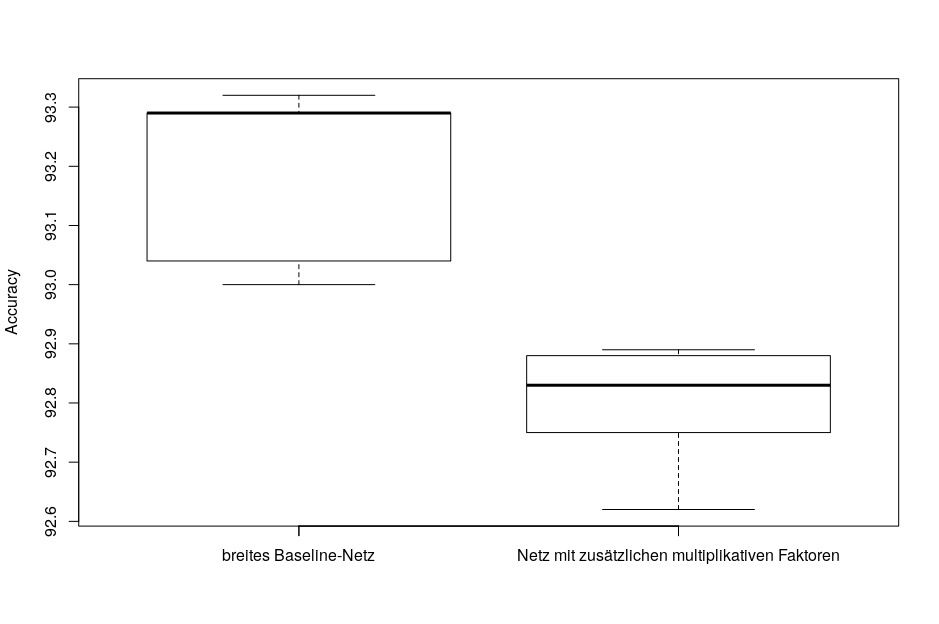
\includegraphics[width= .65\textwidth]{KapitelPartB/Images/baselineMul1.png}\label{abb:BaselineMul1}
     \caption{Vergleich der Accuracy vom Baseline Netz und dem Baseline Netz mit multiplikativen Faktoren}
     \label{abb:BaselineMul}
\end{figure}






\section{Erkunden des Modellraums}
Ausgehende von einem Netz mit drei Blöcken pro Phase $(N=[3,3,3])$, Breite der ersten Schicht von 4 $(K=[4,8,16])$ und einer Schicht pro Block $(l=1)$ werden hintereinander im Abstand von 60 Epochen jeweils ein Operator auf das Netz angewendet. In Abbildung \ref{abb:room1} ist ein Boxplot mit der Accuracy nach der Anwendung jeweils eines Operators zu sehen. Entgegen dem vorherigen Kapitel ergibt sich hier auf für den Operator, der einen Block hinzufügt eine ähnliche Verbesserung wie der Operator für ein breiteres Netz. In den Abbildung \ref{abb:roomw1}, \ref{abb:roomd1} und \ref{abb:roomd21} sind die Boxplots für die Accuracy nach dem Anwenden des zweiten Operators zu sehen. 

 \begin{figure}
     \centering
     \subfloat[][]{\ifx\du\undefined
  \newlength{\du}
\fi
\setlength{\du}{15\unitlength}
\begin{tikzpicture}[even odd rule,scale=0.8]
\pgftransformxscale{1.000000}
\pgftransformyscale{-1.000000}
\definecolor{dialinecolor}{rgb}{0.000000, 0.000000, 0.000000}
\pgfsetstrokecolor{dialinecolor}
\pgfsetstrokeopacity{1.000000}
\definecolor{diafillcolor}{rgb}{1.000000, 1.000000, 1.000000}
\pgfsetfillcolor{diafillcolor}
\pgfsetfillopacity{1.000000}
\pgfsetlinewidth{0.100000\du}
\pgfsetdash{}{0pt}
{\pgfsetcornersarced{\pgfpoint{0.500000\du}{0.500000\du}}\definecolor{diafillcolor}{rgb}{1.000000, 1.000000, 1.000000}
\pgfsetfillcolor{diafillcolor}
\pgfsetfillopacity{1.000000}
\fill (21.546400\du,4.538700\du)--(21.546400\du,6.338700\du)--(25.546400\du,6.338700\du)--(25.546400\du,4.538700\du)--cycle;
}{\pgfsetcornersarced{\pgfpoint{0.500000\du}{0.500000\du}}\definecolor{dialinecolor}{rgb}{0.000000, 0.000000, 0.000000}
\pgfsetstrokecolor{dialinecolor}
\pgfsetstrokeopacity{1.000000}
\draw (21.546400\du,4.538700\du)--(21.546400\du,6.338700\du)--(25.546400\du,6.338700\du)--(25.546400\du,4.538700\du)--cycle;
}% setfont left to latex
\definecolor{dialinecolor}{rgb}{0.000000, 0.000000, 0.000000}
\pgfsetstrokecolor{dialinecolor}
\pgfsetstrokeopacity{1.000000}
\definecolor{diafillcolor}{rgb}{0.000000, 0.000000, 0.000000}
\pgfsetfillcolor{diafillcolor}
\pgfsetfillopacity{1.000000}
\node[anchor=base,inner sep=0pt, outer sep=0pt,color=dialinecolor] at (23.546400\du,5.633700\du){3;16;2};
\pgfsetlinewidth{0.100000\du}
\pgfsetdash{}{0pt}
{\pgfsetcornersarced{\pgfpoint{0.500000\du}{0.500000\du}}\definecolor{diafillcolor}{rgb}{1.000000, 1.000000, 1.000000}
\pgfsetfillcolor{diafillcolor}
\pgfsetfillopacity{1.000000}
\fill (29.501400\du,1.498140\du)--(29.501400\du,3.298140\du)--(33.501400\du,3.298140\du)--(33.501400\du,1.498140\du)--cycle;
}{\pgfsetcornersarced{\pgfpoint{0.500000\du}{0.500000\du}}\definecolor{dialinecolor}{rgb}{0.000000, 0.000000, 0.000000}
\pgfsetstrokecolor{dialinecolor}
\pgfsetstrokeopacity{1.000000}
\draw (29.501400\du,1.498140\du)--(29.501400\du,3.298140\du)--(33.501400\du,3.298140\du)--(33.501400\du,1.498140\du)--cycle;
}% setfont left to latex
\definecolor{dialinecolor}{rgb}{0.000000, 0.000000, 0.000000}
\pgfsetstrokecolor{dialinecolor}
\pgfsetstrokeopacity{1.000000}
\definecolor{diafillcolor}{rgb}{0.000000, 0.000000, 0.000000}
\pgfsetfillcolor{diafillcolor}
\pgfsetfillopacity{1.000000}
\node[anchor=base,inner sep=0pt, outer sep=0pt,color=dialinecolor] at (31.501400\du,2.593140\du){3;8;3};
\pgfsetlinewidth{0.100000\du}
\pgfsetdash{}{0pt}
{\pgfsetcornersarced{\pgfpoint{0.500000\du}{0.500000\du}}\definecolor{diafillcolor}{rgb}{1.000000, 1.000000, 1.000000}
\pgfsetfillcolor{diafillcolor}
\pgfsetfillopacity{1.000000}
\fill (29.572100\du,8.003520\du)--(29.572100\du,9.803520\du)--(33.572100\du,9.803520\du)--(33.572100\du,8.003520\du)--cycle;
}{\pgfsetcornersarced{\pgfpoint{0.500000\du}{0.500000\du}}\definecolor{dialinecolor}{rgb}{0.000000, 0.000000, 0.000000}
\pgfsetstrokecolor{dialinecolor}
\pgfsetstrokeopacity{1.000000}
\draw (29.572100\du,8.003520\du)--(29.572100\du,9.803520\du)--(33.572100\du,9.803520\du)--(33.572100\du,8.003520\du)--cycle;
}% setfont left to latex
\definecolor{dialinecolor}{rgb}{0.000000, 0.000000, 0.000000}
\pgfsetstrokecolor{dialinecolor}
\pgfsetstrokeopacity{1.000000}
\definecolor{diafillcolor}{rgb}{0.000000, 0.000000, 0.000000}
\pgfsetfillcolor{diafillcolor}
\pgfsetfillopacity{1.000000}
\node[anchor=base,inner sep=0pt, outer sep=0pt,color=dialinecolor] at (31.572100\du,9.098520\du){3;8;2};
\pgfsetlinewidth{0.100000\du}
\pgfsetdash{}{0pt}
{\pgfsetcornersarced{\pgfpoint{0.500000\du}{0.500000\du}}\definecolor{diafillcolor}{rgb}{1.000000, 1.000000, 1.000000}
\pgfsetfillcolor{diafillcolor}
\pgfsetfillopacity{1.000000}
\fill (37.244200\du,4.892250\du)--(37.244200\du,6.692250\du)--(41.244200\du,6.692250\du)--(41.244200\du,4.892250\du)--cycle;
}{\pgfsetcornersarced{\pgfpoint{0.500000\du}{0.500000\du}}\definecolor{dialinecolor}{rgb}{0.000000, 0.000000, 0.000000}
\pgfsetstrokecolor{dialinecolor}
\pgfsetstrokeopacity{1.000000}
\draw (37.244200\du,4.892250\du)--(37.244200\du,6.692250\du)--(41.244200\du,6.692250\du)--(41.244200\du,4.892250\du)--cycle;
}% setfont left to latex
\definecolor{dialinecolor}{rgb}{0.000000, 0.000000, 0.000000}
\pgfsetstrokecolor{dialinecolor}
\pgfsetstrokeopacity{1.000000}
\definecolor{diafillcolor}{rgb}{0.000000, 0.000000, 0.000000}
\pgfsetfillcolor{diafillcolor}
\pgfsetfillopacity{1.000000}
\node[anchor=base,inner sep=0pt, outer sep=0pt,color=dialinecolor] at (39.244200\du,5.987250\du){4;8;2};
\pgfsetlinewidth{0.100000\du}
\pgfsetdash{}{0pt}
{\pgfsetcornersarced{\pgfpoint{0.500000\du}{0.500000\du}}\definecolor{diafillcolor}{rgb}{1.000000, 1.000000, 1.000000}
\pgfsetfillcolor{diafillcolor}
\pgfsetfillopacity{1.000000}
\fill (18.435100\du,14.261400\du)--(18.435100\du,16.061400\du)--(22.435100\du,16.061400\du)--(22.435100\du,14.261400\du)--cycle;
}{\pgfsetcornersarced{\pgfpoint{0.500000\du}{0.500000\du}}\definecolor{dialinecolor}{rgb}{0.000000, 0.000000, 0.000000}
\pgfsetstrokecolor{dialinecolor}
\pgfsetstrokeopacity{1.000000}
\draw (18.435100\du,14.261400\du)--(18.435100\du,16.061400\du)--(22.435100\du,16.061400\du)--(22.435100\du,14.261400\du)--cycle;
}% setfont left to latex
\definecolor{dialinecolor}{rgb}{0.000000, 0.000000, 0.000000}
\pgfsetstrokecolor{dialinecolor}
\pgfsetstrokeopacity{1.000000}
\definecolor{diafillcolor}{rgb}{0.000000, 0.000000, 0.000000}
\pgfsetfillcolor{diafillcolor}
\pgfsetfillopacity{1.000000}
\node[anchor=base,inner sep=0pt, outer sep=0pt,color=dialinecolor] at (20.435100\du,15.356400\du){3;8;3};
\pgfsetlinewidth{0.100000\du}
\pgfsetdash{}{0pt}
{\pgfsetcornersarced{\pgfpoint{0.500000\du}{0.500000\du}}\definecolor{diafillcolor}{rgb}{1.000000, 1.000000, 1.000000}
\pgfsetfillcolor{diafillcolor}
\pgfsetfillopacity{1.000000}
\fill (22.006000\du,19.529400\du)--(22.006000\du,21.329400\du)--(26.006000\du,21.329400\du)--(26.006000\du,19.529400\du)--cycle;
}{\pgfsetcornersarced{\pgfpoint{0.500000\du}{0.500000\du}}\definecolor{dialinecolor}{rgb}{0.000000, 0.000000, 0.000000}
\pgfsetstrokecolor{dialinecolor}
\pgfsetstrokeopacity{1.000000}
\draw (22.006000\du,19.529400\du)--(22.006000\du,21.329400\du)--(26.006000\du,21.329400\du)--(26.006000\du,19.529400\du)--cycle;
}% setfont left to latex
\definecolor{dialinecolor}{rgb}{0.000000, 0.000000, 0.000000}
\pgfsetstrokecolor{dialinecolor}
\pgfsetstrokeopacity{1.000000}
\definecolor{diafillcolor}{rgb}{0.000000, 0.000000, 0.000000}
\pgfsetfillcolor{diafillcolor}
\pgfsetfillopacity{1.000000}
\node[anchor=base,inner sep=0pt, outer sep=0pt,color=dialinecolor] at (24.006000\du,20.624400\du){3;4;3};
\pgfsetlinewidth{0.100000\du}
\pgfsetdash{}{0pt}
{\pgfsetcornersarced{\pgfpoint{0.500000\du}{0.500000\du}}\definecolor{diafillcolor}{rgb}{1.000000, 1.000000, 1.000000}
\pgfsetfillcolor{diafillcolor}
\pgfsetfillopacity{1.000000}
\fill (17.233100\du,25.442500\du)--(17.233100\du,27.242500\du)--(21.233100\du,27.242500\du)--(21.233100\du,25.442500\du)--cycle;
}{\pgfsetcornersarced{\pgfpoint{0.500000\du}{0.500000\du}}\definecolor{dialinecolor}{rgb}{0.000000, 0.000000, 0.000000}
\pgfsetstrokecolor{dialinecolor}
\pgfsetstrokeopacity{1.000000}
\draw (17.233100\du,25.442500\du)--(17.233100\du,27.242500\du)--(21.233100\du,27.242500\du)--(21.233100\du,25.442500\du)--cycle;
}% setfont left to latex
\definecolor{dialinecolor}{rgb}{0.000000, 0.000000, 0.000000}
\pgfsetstrokecolor{dialinecolor}
\pgfsetstrokeopacity{1.000000}
\definecolor{diafillcolor}{rgb}{0.000000, 0.000000, 0.000000}
\pgfsetfillcolor{diafillcolor}
\pgfsetfillopacity{1.000000}
\node[anchor=base,inner sep=0pt, outer sep=0pt,color=dialinecolor] at (19.233100\du,26.537500\du){3;4;4};
\pgfsetlinewidth{0.100000\du}
\pgfsetdash{}{0pt}
{\pgfsetcornersarced{\pgfpoint{0.500000\du}{0.500000\du}}\definecolor{diafillcolor}{rgb}{1.000000, 1.000000, 1.000000}
\pgfsetfillcolor{diafillcolor}
\pgfsetfillopacity{1.000000}
\fill (25.930500\du,24.982900\du)--(25.930500\du,26.782900\du)--(29.930500\du,26.782900\du)--(29.930500\du,24.982900\du)--cycle;
}{\pgfsetcornersarced{\pgfpoint{0.500000\du}{0.500000\du}}\definecolor{dialinecolor}{rgb}{0.000000, 0.000000, 0.000000}
\pgfsetstrokecolor{dialinecolor}
\pgfsetstrokeopacity{1.000000}
\draw (25.930500\du,24.982900\du)--(25.930500\du,26.782900\du)--(29.930500\du,26.782900\du)--(29.930500\du,24.982900\du)--cycle;
}% setfont left to latex
\definecolor{dialinecolor}{rgb}{0.000000, 0.000000, 0.000000}
\pgfsetstrokecolor{dialinecolor}
\pgfsetstrokeopacity{1.000000}
\definecolor{diafillcolor}{rgb}{0.000000, 0.000000, 0.000000}
\pgfsetfillcolor{diafillcolor}
\pgfsetfillopacity{1.000000}
\node[anchor=base,inner sep=0pt, outer sep=0pt,color=dialinecolor] at (27.930500\du,26.077900\du){4;4;3};
\pgfsetlinewidth{0.100000\du}
\pgfsetdash{}{0pt}
{\pgfsetcornersarced{\pgfpoint{0.500000\du}{0.500000\du}}\definecolor{diafillcolor}{rgb}{1.000000, 1.000000, 1.000000}
\pgfsetfillcolor{diafillcolor}
\pgfsetfillopacity{1.000000}
\fill (43.784900\du,14.199500\du)--(43.784900\du,15.999500\du)--(47.784900\du,15.999500\du)--(47.784900\du,14.199500\du)--cycle;
}{\pgfsetcornersarced{\pgfpoint{0.500000\du}{0.500000\du}}\definecolor{dialinecolor}{rgb}{0.000000, 0.000000, 0.000000}
\pgfsetstrokecolor{dialinecolor}
\pgfsetstrokeopacity{1.000000}
\draw (43.784900\du,14.199500\du)--(43.784900\du,15.999500\du)--(47.784900\du,15.999500\du)--(47.784900\du,14.199500\du)--cycle;
}% setfont left to latex
\definecolor{dialinecolor}{rgb}{0.000000, 0.000000, 0.000000}
\pgfsetstrokecolor{dialinecolor}
\pgfsetstrokeopacity{1.000000}
\definecolor{diafillcolor}{rgb}{0.000000, 0.000000, 0.000000}
\pgfsetfillcolor{diafillcolor}
\pgfsetfillopacity{1.000000}
\node[anchor=base,inner sep=0pt, outer sep=0pt,color=dialinecolor] at (45.784900\du,15.294500\du){4;4;3};
\pgfsetlinewidth{0.100000\du}
\pgfsetdash{}{0pt}
{\pgfsetcornersarced{\pgfpoint{0.500000\du}{0.500000\du}}\definecolor{diafillcolor}{rgb}{1.000000, 1.000000, 1.000000}
\pgfsetfillcolor{diafillcolor}
\pgfsetfillopacity{1.000000}
\fill (45.694100\du,24.841500\du)--(45.694100\du,26.641500\du)--(49.694100\du,26.641500\du)--(49.694100\du,24.841500\du)--cycle;
}{\pgfsetcornersarced{\pgfpoint{0.500000\du}{0.500000\du}}\definecolor{dialinecolor}{rgb}{0.000000, 0.000000, 0.000000}
\pgfsetstrokecolor{dialinecolor}
\pgfsetstrokeopacity{1.000000}
\draw (45.694100\du,24.841500\du)--(45.694100\du,26.641500\du)--(49.694100\du,26.641500\du)--(49.694100\du,24.841500\du)--cycle;
}% setfont left to latex
\definecolor{dialinecolor}{rgb}{0.000000, 0.000000, 0.000000}
\pgfsetstrokecolor{dialinecolor}
\pgfsetstrokeopacity{1.000000}
\definecolor{diafillcolor}{rgb}{0.000000, 0.000000, 0.000000}
\pgfsetfillcolor{diafillcolor}
\pgfsetfillopacity{1.000000}
\node[anchor=base,inner sep=0pt, outer sep=0pt,color=dialinecolor] at (47.694100\du,25.936500\du){5;4;2};
\pgfsetlinewidth{0.100000\du}
\pgfsetdash{}{0pt}
{\pgfsetcornersarced{\pgfpoint{0.500000\du}{0.500000\du}}\definecolor{diafillcolor}{rgb}{1.000000, 1.000000, 1.000000}
\pgfsetfillcolor{diafillcolor}
\pgfsetfillopacity{1.000000}
\fill (36.431000\du,24.912200\du)--(36.431000\du,26.712200\du)--(40.431000\du,26.712200\du)--(40.431000\du,24.912200\du)--cycle;
}{\pgfsetcornersarced{\pgfpoint{0.500000\du}{0.500000\du}}\definecolor{dialinecolor}{rgb}{0.000000, 0.000000, 0.000000}
\pgfsetstrokecolor{dialinecolor}
\pgfsetstrokeopacity{1.000000}
\draw (36.431000\du,24.912200\du)--(36.431000\du,26.712200\du)--(40.431000\du,26.712200\du)--(40.431000\du,24.912200\du)--cycle;
}% setfont left to latex
\definecolor{dialinecolor}{rgb}{0.000000, 0.000000, 0.000000}
\pgfsetstrokecolor{dialinecolor}
\pgfsetstrokeopacity{1.000000}
\definecolor{diafillcolor}{rgb}{0.000000, 0.000000, 0.000000}
\pgfsetfillcolor{diafillcolor}
\pgfsetfillopacity{1.000000}
\node[anchor=base,inner sep=0pt, outer sep=0pt,color=dialinecolor] at (38.431000\du,26.007200\du){4;8;2};
\pgfsetlinewidth{0.100000\du}
\pgfsetdash{}{0pt}
{\pgfsetcornersarced{\pgfpoint{0.500000\du}{0.500000\du}}\definecolor{diafillcolor}{rgb}{1.000000, 1.000000, 1.000000}
\pgfsetfillcolor{diafillcolor}
\pgfsetfillopacity{1.000000}
\fill (29.572100\du,15.056900\du)--(29.572100\du,16.856900\du)--(33.572100\du,16.856900\du)--(33.572100\du,15.056900\du)--cycle;
}{\pgfsetcornersarced{\pgfpoint{0.500000\du}{0.500000\du}}\definecolor{dialinecolor}{rgb}{0.000000, 0.000000, 0.000000}
\pgfsetstrokecolor{dialinecolor}
\pgfsetstrokeopacity{1.000000}
\draw (29.572100\du,15.056900\du)--(29.572100\du,16.856900\du)--(33.572100\du,16.856900\du)--(33.572100\du,15.056900\du)--cycle;
}% setfont left to latex
\definecolor{dialinecolor}{rgb}{0.000000, 0.000000, 0.000000}
\pgfsetstrokecolor{dialinecolor}
\pgfsetstrokeopacity{1.000000}
\definecolor{diafillcolor}{rgb}{0.000000, 0.000000, 0.000000}
\pgfsetfillcolor{diafillcolor}
\pgfsetfillopacity{1.000000}
\node[anchor=base,inner sep=0pt, outer sep=0pt,color=dialinecolor] at (31.572100\du,16.151900\du){3;4;2};
\pgfsetlinewidth{0.100000\du}
\pgfsetdash{}{0pt}
{\pgfsetcornersarced{\pgfpoint{0.500000\du}{0.500000\du}}\definecolor{diafillcolor}{rgb}{1.000000, 1.000000, 1.000000}
\pgfsetfillcolor{diafillcolor}
\pgfsetfillopacity{1.000000}
\fill (38.623000\du,19.361400\du)--(38.623000\du,21.161400\du)--(42.623000\du,21.161400\du)--(42.623000\du,19.361400\du)--cycle;
}{\pgfsetcornersarced{\pgfpoint{0.500000\du}{0.500000\du}}\definecolor{dialinecolor}{rgb}{0.000000, 0.000000, 0.000000}
\pgfsetstrokecolor{dialinecolor}
\pgfsetstrokeopacity{1.000000}
\draw (38.623000\du,19.361400\du)--(38.623000\du,21.161400\du)--(42.623000\du,21.161400\du)--(42.623000\du,19.361400\du)--cycle;
}% setfont left to latex
\definecolor{dialinecolor}{rgb}{0.000000, 0.000000, 0.000000}
\pgfsetstrokecolor{dialinecolor}
\pgfsetstrokeopacity{1.000000}
\definecolor{diafillcolor}{rgb}{0.000000, 0.000000, 0.000000}
\pgfsetfillcolor{diafillcolor}
\pgfsetfillopacity{1.000000}
\node[anchor=base,inner sep=0pt, outer sep=0pt,color=dialinecolor] at (40.623000\du,20.456400\du){4;4;2};
\pgfsetlinewidth{0.100000\du}
\pgfsetdash{}{0pt}
\pgfsetbuttcap
{
\definecolor{diafillcolor}{rgb}{0.000000, 0.000000, 0.000000}
\pgfsetfillcolor{diafillcolor}
\pgfsetfillopacity{1.000000}
% was here!!!
\pgfsetarrowsend{stealth}
\definecolor{dialinecolor}{rgb}{0.000000, 0.000000, 0.000000}
\pgfsetstrokecolor{dialinecolor}
\pgfsetstrokeopacity{1.000000}
\draw (29.522078\du,8.018494\du)--(25.596422\du,6.323726\du);
}
\pgfsetlinewidth{0.100000\du}
\pgfsetdash{}{0pt}
\pgfsetbuttcap
{
\definecolor{diafillcolor}{rgb}{0.000000, 0.000000, 0.000000}
\pgfsetfillcolor{diafillcolor}
\pgfsetfillopacity{1.000000}
% was here!!!
\pgfsetarrowsend{stealth}
\definecolor{dialinecolor}{rgb}{0.000000, 0.000000, 0.000000}
\pgfsetstrokecolor{dialinecolor}
\pgfsetstrokeopacity{1.000000}
\draw (31.561774\du,7.953363\du)--(31.511726\du,3.348297\du);
}
\pgfsetlinewidth{0.100000\du}
\pgfsetdash{}{0pt}
\pgfsetbuttcap
{
\definecolor{diafillcolor}{rgb}{0.000000, 0.000000, 0.000000}
\pgfsetfillcolor{diafillcolor}
\pgfsetfillopacity{1.000000}
% was here!!!
\pgfsetarrowsend{stealth}
\definecolor{dialinecolor}{rgb}{0.000000, 0.000000, 0.000000}
\pgfsetstrokecolor{dialinecolor}
\pgfsetstrokeopacity{1.000000}
\draw (33.572100\du,8.903520\du)--(37.512520\du,6.742114\du);
}
\pgfsetlinewidth{0.100000\du}
\pgfsetdash{}{0pt}
\pgfsetbuttcap
{
\definecolor{diafillcolor}{rgb}{0.000000, 0.000000, 0.000000}
\pgfsetfillcolor{diafillcolor}
\pgfsetfillopacity{1.000000}
% was here!!!
\pgfsetarrowsend{stealth}
\definecolor{dialinecolor}{rgb}{0.000000, 0.000000, 0.000000}
\pgfsetstrokecolor{dialinecolor}
\pgfsetstrokeopacity{1.000000}
\draw (31.572100\du,15.013235\du)--(31.572100\du,9.847185\du);
}
\pgfsetlinewidth{0.100000\du}
\pgfsetdash{}{0pt}
\pgfsetbuttcap
{
\definecolor{diafillcolor}{rgb}{0.000000, 0.000000, 0.000000}
\pgfsetfillcolor{diafillcolor}
\pgfsetfillopacity{1.000000}
% was here!!!
\pgfsetarrowsend{stealth}
\definecolor{dialinecolor}{rgb}{0.000000, 0.000000, 0.000000}
\pgfsetstrokecolor{dialinecolor}
\pgfsetstrokeopacity{1.000000}
\draw (29.964581\du,16.907142\du)--(25.613519\du,19.479158\du);
}
\pgfsetlinewidth{0.100000\du}
\pgfsetdash{}{0pt}
\pgfsetbuttcap
{
\definecolor{diafillcolor}{rgb}{0.000000, 0.000000, 0.000000}
\pgfsetfillcolor{diafillcolor}
\pgfsetfillopacity{1.000000}
% was here!!!
\pgfsetarrowsend{stealth}
\definecolor{dialinecolor}{rgb}{0.000000, 0.000000, 0.000000}
\pgfsetstrokecolor{dialinecolor}
\pgfsetstrokeopacity{1.000000}
\draw (24.006000\du,19.529400\du)--(21.211439\du,16.111035\du);
}
\pgfsetlinewidth{0.100000\du}
\pgfsetdash{}{0pt}
\pgfsetbuttcap
{
\definecolor{diafillcolor}{rgb}{0.000000, 0.000000, 0.000000}
\pgfsetfillcolor{diafillcolor}
\pgfsetfillopacity{1.000000}
% was here!!!
\pgfsetarrowsend{stealth}
\definecolor{dialinecolor}{rgb}{0.000000, 0.000000, 0.000000}
\pgfsetstrokecolor{dialinecolor}
\pgfsetstrokeopacity{1.000000}
\draw (23.238968\du,21.379668\du)--(20.000132\du,25.392232\du);
}
\pgfsetlinewidth{0.100000\du}
\pgfsetdash{}{0pt}
\pgfsetbuttcap
{
\definecolor{diafillcolor}{rgb}{0.000000, 0.000000, 0.000000}
\pgfsetfillcolor{diafillcolor}
\pgfsetfillopacity{1.000000}
% was here!!!
\pgfsetarrowsend{stealth}
\definecolor{dialinecolor}{rgb}{0.000000, 0.000000, 0.000000}
\pgfsetstrokecolor{dialinecolor}
\pgfsetstrokeopacity{1.000000}
\draw (24.689147\du,21.378703\du)--(27.247353\du,24.933597\du);
}
\pgfsetlinewidth{0.100000\du}
\pgfsetdash{}{0pt}
\pgfsetbuttcap
{
\definecolor{diafillcolor}{rgb}{0.000000, 0.000000, 0.000000}
\pgfsetfillcolor{diafillcolor}
\pgfsetfillopacity{1.000000}
% was here!!!
\pgfsetarrowsend{stealth}
\definecolor{dialinecolor}{rgb}{0.000000, 0.000000, 0.000000}
\pgfsetstrokecolor{dialinecolor}
\pgfsetstrokeopacity{1.000000}
\draw (33.560823\du,16.902713\du)--(38.634277\du,19.315587\du);
}
\pgfsetlinewidth{0.100000\du}
\pgfsetdash{}{0pt}
\pgfsetbuttcap
{
\definecolor{diafillcolor}{rgb}{0.000000, 0.000000, 0.000000}
\pgfsetfillcolor{diafillcolor}
\pgfsetfillopacity{1.000000}
% was here!!!
\pgfsetarrowsend{stealth}
\definecolor{dialinecolor}{rgb}{0.000000, 0.000000, 0.000000}
\pgfsetstrokecolor{dialinecolor}
\pgfsetstrokeopacity{1.000000}
\draw (42.158600\du,19.149300\du)--(44.934543\du,16.049166\du);
}
\pgfsetlinewidth{0.100000\du}
\pgfsetdash{}{0pt}
\pgfsetbuttcap
{
\definecolor{diafillcolor}{rgb}{0.000000, 0.000000, 0.000000}
\pgfsetfillcolor{diafillcolor}
\pgfsetfillopacity{1.000000}
% was here!!!
\pgfsetarrowsend{stealth}
\definecolor{dialinecolor}{rgb}{0.000000, 0.000000, 0.000000}
\pgfsetstrokecolor{dialinecolor}
\pgfsetstrokeopacity{1.000000}
\draw (41.849135\du,21.211654\du)--(46.467965\du,24.791246\du);
}
\pgfsetlinewidth{0.100000\du}
\pgfsetdash{}{0pt}
\pgfsetbuttcap
{
\definecolor{diafillcolor}{rgb}{0.000000, 0.000000, 0.000000}
\pgfsetfillcolor{diafillcolor}
\pgfsetfillopacity{1.000000}
% was here!!!
\pgfsetarrowsend{stealth}
\definecolor{dialinecolor}{rgb}{0.000000, 0.000000, 0.000000}
\pgfsetstrokecolor{dialinecolor}
\pgfsetstrokeopacity{1.000000}
\draw (40.247722\du,21.211717\du)--(38.806278\du,24.861883\du);
}
% setfont left to latex
\definecolor{dialinecolor}{rgb}{0.000000, 0.000000, 0.000000}
\pgfsetstrokecolor{dialinecolor}
\pgfsetstrokeopacity{1.000000}
\definecolor{diafillcolor}{rgb}{0.000000, 0.000000, 0.000000}
\pgfsetfillcolor{diafillcolor}
\pgfsetfillopacity{1.000000}
\node[anchor=base west,inner sep=0pt,outer sep=0pt,color=dialinecolor] at (25.506200\du,7.649970\du){Breiter};
% setfont left to latex
\definecolor{dialinecolor}{rgb}{0.000000, 0.000000, 0.000000}
\pgfsetstrokecolor{dialinecolor}
\pgfsetstrokeopacity{1.000000}
\definecolor{diafillcolor}{rgb}{0.000000, 0.000000, 0.000000}
\pgfsetfillcolor{diafillcolor}
\pgfsetfillopacity{1.000000}
\node[anchor=base west,inner sep=0pt,outer sep=0pt,color=dialinecolor] at (30.562000\du,5.033670\du){Tiefer 1};
% setfont left to latex
\definecolor{dialinecolor}{rgb}{0.000000, 0.000000, 0.000000}
\pgfsetstrokecolor{dialinecolor}
\pgfsetstrokeopacity{1.000000}
\definecolor{diafillcolor}{rgb}{0.000000, 0.000000, 0.000000}
\pgfsetfillcolor{diafillcolor}
\pgfsetfillopacity{1.000000}
\node[anchor=base west,inner sep=0pt,outer sep=0pt,color=dialinecolor] at (35.441100\du,7.261060\du){Tiefer 2};
% setfont left to latex
\definecolor{dialinecolor}{rgb}{0.000000, 0.000000, 0.000000}
\pgfsetstrokecolor{dialinecolor}
\pgfsetstrokeopacity{1.000000}
\definecolor{diafillcolor}{rgb}{0.000000, 0.000000, 0.000000}
\pgfsetfillcolor{diafillcolor}
\pgfsetfillopacity{1.000000}
\node[anchor=base west,inner sep=0pt,outer sep=0pt,color=dialinecolor] at (31.926700\du,11.208500\du){Breiter};
% setfont left to latex
\definecolor{dialinecolor}{rgb}{0.000000, 0.000000, 0.000000}
\pgfsetstrokecolor{dialinecolor}
\pgfsetstrokeopacity{1.000000}
\definecolor{diafillcolor}{rgb}{0.000000, 0.000000, 0.000000}
\pgfsetfillcolor{diafillcolor}
\pgfsetfillopacity{1.000000}
\node[anchor=base west,inner sep=0pt,outer sep=0pt,color=dialinecolor] at (26.517400\du,17.996700\du){Tiefer 1};
% setfont left to latex
\definecolor{dialinecolor}{rgb}{0.000000, 0.000000, 0.000000}
\pgfsetstrokecolor{dialinecolor}
\pgfsetstrokeopacity{1.000000}
\definecolor{diafillcolor}{rgb}{0.000000, 0.000000, 0.000000}
\pgfsetfillcolor{diafillcolor}
\pgfsetfillopacity{1.000000}
\node[anchor=base west,inner sep=0pt,outer sep=0pt,color=dialinecolor] at (36.346200\du,17.784600\du){Tiefer 2};
% setfont left to latex
\definecolor{dialinecolor}{rgb}{0.000000, 0.000000, 0.000000}
\pgfsetstrokecolor{dialinecolor}
\pgfsetstrokeopacity{1.000000}
\definecolor{diafillcolor}{rgb}{0.000000, 0.000000, 0.000000}
\pgfsetfillcolor{diafillcolor}
\pgfsetfillopacity{1.000000}
\node[anchor=base west,inner sep=0pt,outer sep=0pt,color=dialinecolor] at (22.359600\du,17.195900\du){Breiter};
% setfont left to latex
\definecolor{dialinecolor}{rgb}{0.000000, 0.000000, 0.000000}
\pgfsetstrokecolor{dialinecolor}
\pgfsetstrokeopacity{1.000000}
\definecolor{diafillcolor}{rgb}{0.000000, 0.000000, 0.000000}
\pgfsetfillcolor{diafillcolor}
\pgfsetfillopacity{1.000000}
\node[anchor=base west,inner sep=0pt,outer sep=0pt,color=dialinecolor] at (19.573600\du,24.242200\du){Tiefer 1};
% setfont left to latex
\definecolor{dialinecolor}{rgb}{0.000000, 0.000000, 0.000000}
\pgfsetstrokecolor{dialinecolor}
\pgfsetstrokeopacity{1.000000}
\definecolor{diafillcolor}{rgb}{0.000000, 0.000000, 0.000000}
\pgfsetfillcolor{diafillcolor}
\pgfsetfillopacity{1.000000}
\node[anchor=base west,inner sep=0pt,outer sep=0pt,color=dialinecolor] at (26.821400\du,23.818000\du){Tiefer 2};
% setfont left to latex
\definecolor{dialinecolor}{rgb}{0.000000, 0.000000, 0.000000}
\pgfsetstrokecolor{dialinecolor}
\pgfsetstrokeopacity{1.000000}
\definecolor{diafillcolor}{rgb}{0.000000, 0.000000, 0.000000}
\pgfsetfillcolor{diafillcolor}
\pgfsetfillopacity{1.000000}
\node[anchor=base west,inner sep=0pt,outer sep=0pt,color=dialinecolor] at (38.361400\du,23.936400\du){Breiter};
% setfont left to latex
\definecolor{dialinecolor}{rgb}{0.000000, 0.000000, 0.000000}
\pgfsetstrokecolor{dialinecolor}
\pgfsetstrokeopacity{1.000000}
\definecolor{diafillcolor}{rgb}{0.000000, 0.000000, 0.000000}
\pgfsetfillcolor{diafillcolor}
\pgfsetfillopacity{1.000000}
\node[anchor=base west,inner sep=0pt,outer sep=0pt,color=dialinecolor] at (42.696000\du,17.454000\du){Tiefer 1};
% setfont left to latex
\definecolor{dialinecolor}{rgb}{0.000000, 0.000000, 0.000000}
\pgfsetstrokecolor{dialinecolor}
\pgfsetstrokeopacity{1.000000}
\definecolor{diafillcolor}{rgb}{0.000000, 0.000000, 0.000000}
\pgfsetfillcolor{diafillcolor}
\pgfsetfillopacity{1.000000}
\node[anchor=base west,inner sep=0pt,outer sep=0pt,color=dialinecolor] at (45.029400\du,23.181600\du){Tiefer 2};
\end{tikzpicture}

     \label{abb:deeperRoom1}}
     \caption{Übersicht über die Anwendung der Operatoren auf das Ausgangsnetz. Beschriftung der Knoten: \{Anzahl an Blöcken pro Phase; Breite der ersten Schicht; Schichten pro Block \}. Tiefer 1 bezeichnet den Operator, der jedem Block eine zusätzliche Schicht hinzufügt. Tiefer 2 bezeichnet den Operator, der jeder Phase einen zusätzlichen Block hinzufügt.}
     \hfill
\end{figure}

Es fällt auf, dass die Reihenfolge, in welcher die Operatoren angewendet werden einen großen Unterschied machen. Außerdem hat jeder Zweig des Baumes, nachdem Anwenden des ersten Operators zumindest ein Blatt, bei dem die Accuracy zugenommen hat.

\begin{figure}
     \centering
     \subfloat[][Anwendung des ersten Operators]{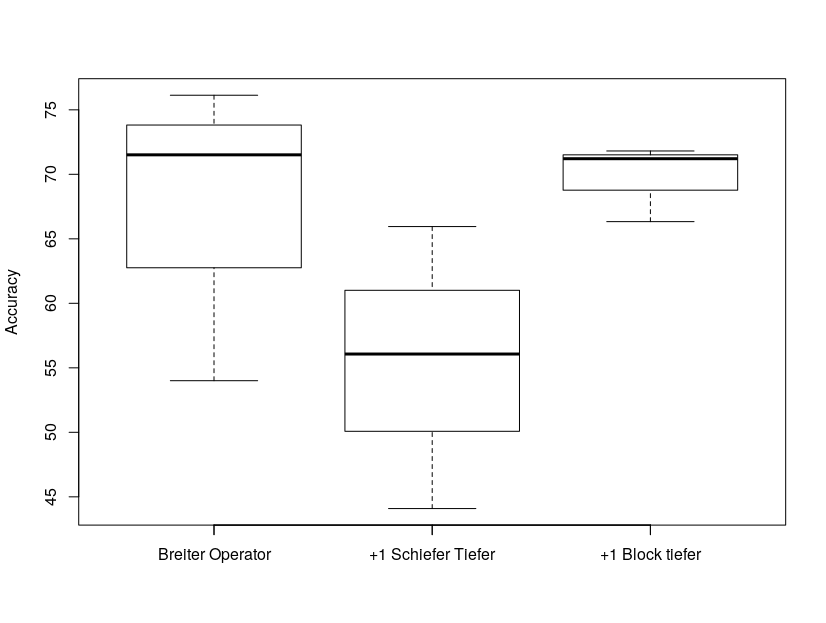
\includegraphics[width= .47\textwidth]{KapitelPartB/Images/room1.png}\label{abb:room1}}     
     \subfloat[][Anwendung des zweiten Operators nach Anwenden des Operators für ein breiteres Netz]{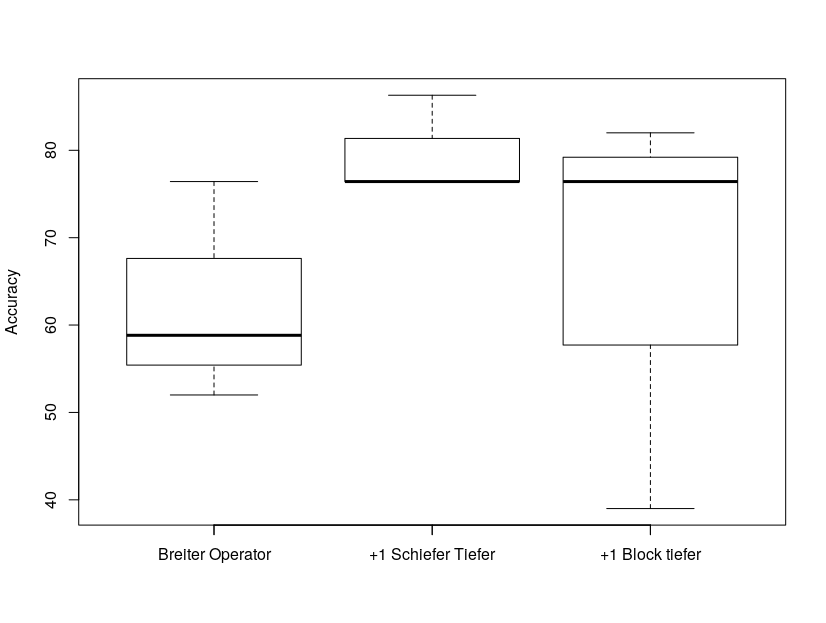
\includegraphics[width= .47\textwidth]{KapitelPartB/Images/roomw1.png}\label{abb:roomw1}}
     \hfill
     \subfloat[][Anwendung des zweiten Operators nach Anwenden des Operators für ein Netz mit einer zusätzlichen Schicht pro Block]{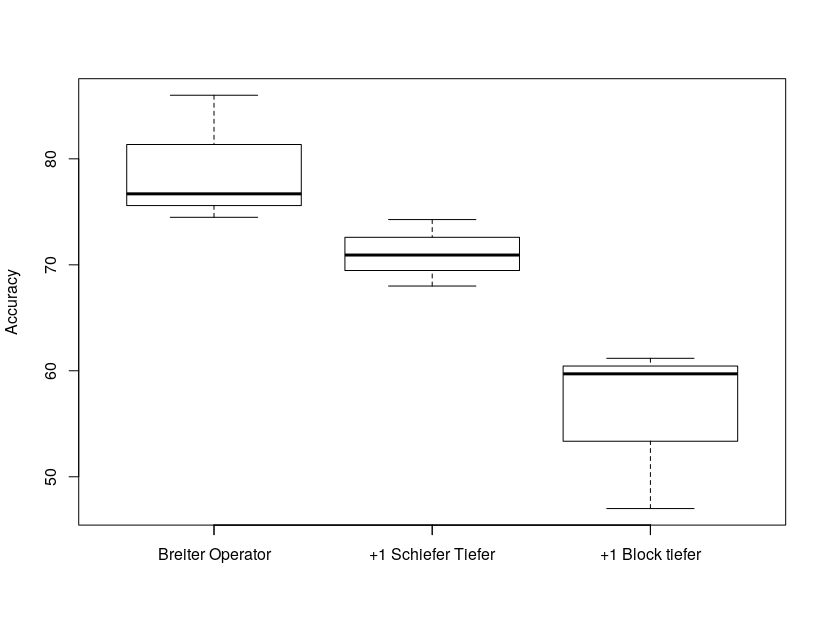
\includegraphics[width= .47\textwidth]{KapitelPartB/Images/roomd1.png}\label{abb:roomd1}}
     \subfloat[][Anwendung des zweiten Operators nach Anwenden des Operators für ein Netz mit einem zusätzlichen Block pro Phase]{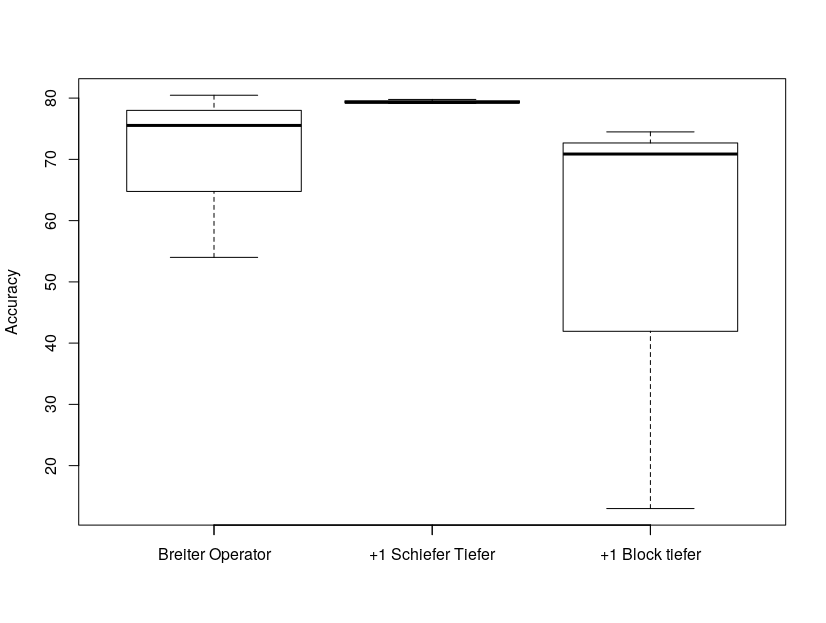
\includegraphics[width= .47\textwidth]{KapitelPartB/Images/roomd21.png}\label{abb:roomd21}}

     \caption{}
     \label{abb:room}
\end{figure}
 Obwohl das Ausgangsnetz hier sehr klein ist gibt es durch das Anwenden der Operatoren ein Verbesserungspotential bei den meisten Operatoren.
